\chapter{Thực nghiệm và đánh giá}
\label{ch:thuc-nghiem}

\section{Môi trường thực nghiệm}
\label{sec:moi-truong-thuc-nghiem}

Để đảm bảo tính khả lập (reproducibility) và tính minh bạch tuyệt đối của toàn bộ quá trình nghiên cứu, tất cả các thực nghiệm trong framework DepSev-ML được thực thi trên môi trường phần cứng và phần mềm chuẩn tắc:
\begin{itemize}
    \item \textbf{Phần cứng (Hardware):} Máy trạm cá nhân Apple Silicon (kiến trúc ARM64, vi xử lý Apple M-series), bộ nhớ RAM 16 GB, ổ cứng thể rắn SSD tốc độ cao.
    \item \textbf{Hệ điều hành (Operating System):} macOS (Darwin Kernel Version 24.6.0).
    \item \textbf{Môi trường phần mềm và Ngôn ngữ lập trình:} Python phiên bản 3.13.7 (Clang 16.0.0) chạy trong môi trường ảo hóa độc lập (\texttt{.venv}).
    \item \textbf{Các thư viện tính toán khoa học cốt lõi:}
    \begin{itemize}
        \item \texttt{scikit-learn}: Phiên bản 1.9.1 (cung cấp các thuật toán nền tảng, tiền xử lý, kiểm định chéo và các độ đo đánh giá).
        \item \texttt{numpy}: Phiên bản 2.5.3 (xử lý ma trận và tính toán đại số tuyến tính tối ưu hóa).
        \item \texttt{pandas}: Phiên bản 3.0.6 (quản lý, lọc và biến đổi dữ liệu dạng bảng).
        \item \texttt{scipy}: Phiên bản 1.18.1 (tối ưu hóa phi tuyến bậc hai L-BFGS-B cho mô hình Ordinal Logistic Regression).
        \item \texttt{xgboost}: Phiên bản 3.4.1 (thuật toán eXtreme Gradient Boosting với hỗ trợ trọng số lớp động).
        \item \texttt{matplotlib} (3.11.2) và \texttt{seaborn}: Trực quan hóa dữ liệu và xuất bản biểu đồ khoa học độ phân giải cao (300 DPI).
    \end{itemize}
    \item \textbf{Quản lý hạt giống ngẫu nhiên (Random Seed Control):} Tham số \texttt{random\_state = 42} được cố định nghiêm ngặt trên toàn bộ các phép chia fold, khởi tạo mô hình và lấy mẫu bootstrap nhằm triệt tiêu phương sai ngẫu nhiên giữa các lần chạy.
\end{itemize}

\section{Thực nghiệm Baseline và Cắt bỏ đặc trưng (Feature Ablation)}
\label{sec:feature-ablation}

\subsection{Mục tiêu và thiết lập thực nghiệm}
Thực nghiệm Feature Ablation nhằm trả lời câu hỏi nghiên cứu \textbf{RQ1}: Khảo sát sự đóng góp thực tế của bốn nhóm đặc trưng lũy tiến ($F_1 \to F_4$) đối với khả năng dự đoán mức độ PHQ-9 (nhiệm vụ 5 lớp $T_5$: $C_0 \to C_4$). Thực nghiệm được thực hiện thông qua Stratified 5-Fold Cross-Validation trên tập Legacy Development Cohort ($N = 4.045$). Bốn thuật toán học máy cơ sở được đánh giá song song: Hồi quy Logistic (LR), Cây quyết định (DT), Rừng ngẫu nhiên (RF) và eXtreme Gradient Boosting (XGBoost).

\subsection{Kết quả thực nghiệm}
Số liệu out-of-fold chi tiết được trích xuất từ file kết quả gốc \texttt{results/tables/feature\_ablation\_results\_final\_protocol.csv} và được tổng hợp trong Bảng \ref{tab:ablation-results}. Hình \ref{fig:ablation-comparison} trực quan hóa xu hướng biến thiên Macro-F1 và Balanced Accuracy.

\begin{table}{Kết quả thực nghiệm Feature Ablation trên tập Legacy Development ($N = 4.045$, 5 lớp $T_5$)}
\centering
\label{tab:ablation-results}
\begin{tabular}{l c c c c c}
\toprule
\textbf{Nhóm đặc trưng} & \textbf{Số biến ($d$)} & \textbf{Mô hình ML} & \textbf{Macro-F1 (Mean $\pm$ SD)} & \textbf{Balanced Acc} & \textbf{Weighted-F1} \\
\midrule
\multirow{4}{*}{\textbf{$F_1$} (Thể chất \& Sinh tồn)} & \multirow{4}{*}{10} 
  & Logistic Regression & 0.1899 $\pm$ 0.0164 & 0.2420 $\pm$ 0.0299 & 0.4926 $\pm$ 0.0209 \\
& & Decision Tree        & 0.2081 $\pm$ 0.0121 & 0.2090 $\pm$ 0.0133 & 0.5926 $\pm$ 0.0081 \\
& & Random Forest       & 0.2052 $\pm$ 0.0072 & 0.2090 $\pm$ 0.0065 & 0.6314 $\pm$ 0.0107 \\
& & XGBoost             & 0.2173 $\pm$ 0.0147 & 0.2295 $\pm$ 0.0220 & 0.5577 $\pm$ 0.0072 \\
\midrule
\multirow{4}{*}{\textbf{$F_2$} ($F_1$ + Xét nghiệm máu)} & \multirow{4}{*}{19} 
  & Logistic Regression & 0.2338 $\pm$ 0.0041 & 0.2942 $\pm$ 0.0299 & 0.5648 $\pm$ 0.0092 \\
& & Decision Tree        & 0.2319 $\pm$ 0.0154 & 0.2358 $\pm$ 0.0185 & 0.6144 $\pm$ 0.0093 \\
& & Random Forest       & 0.2350 $\pm$ 0.0180 & 0.2353 $\pm$ 0.0155 & 0.6557 $\pm$ 0.0097 \\
& & XGBoost             & 0.2447 $\pm$ 0.0143 & 0.2594 $\pm$ 0.0187 & 0.6002 $\pm$ 0.0123 \\
\midrule
\multirow{4}{*}{\textbf{$F_3$} ($F_2$ + Lối sống)} & \multirow{4}{*}{29} 
  & Logistic Regression & 0.2390 $\pm$ 0.0084 & 0.3194 $\pm$ 0.0284 & 0.5637 $\pm$ 0.0071 \\
& & Decision Tree        & 0.2388 $\pm$ 0.0127 & 0.2408 $\pm$ 0.0148 & 0.6195 $\pm$ 0.0100 \\
& & Random Forest       & 0.2299 $\pm$ 0.0045 & 0.2314 $\pm$ 0.0047 & 0.6657 $\pm$ 0.0085 \\
& & XGBoost             & 0.2588 $\pm$ 0.0402 & 0.2713 $\pm$ 0.0490 & 0.6112 $\pm$ 0.0154 \\
\midrule
\multirow{4}{*}{\textbf{$F_4$} ($F_3$ + Nhân khẩu học)} & \multirow{4}{*}{34} 
  & Logistic Regression & 0.2399 $\pm$ 0.0148 & \textbf{0.3216 $\pm$ 0.0508} & 0.5642 $\pm$ 0.0112 \\
& & Decision Tree        & 0.2412 $\pm$ 0.0175 & 0.2450 $\pm$ 0.0206 & 0.6214 $\pm$ 0.0098 \\
& & Random Forest       & 0.2232 $\pm$ 0.0099 & 0.2253 $\pm$ 0.0075 & \textbf{0.6728 $\pm$ 0.0091} \\
& & XGBoost             & \textbf{0.2707 $\pm$ 0.0428} & 0.2837 $\pm$ 0.0485 & 0.6384 $\pm$ 0.0148 \\
\bottomrule
\end{tabular}
\end{table}

\begin{figure}{So sánh hiệu năng Macro-F1 của 4 thuật toán trên các nhóm đặc trưng lũy tiến $F_1 \to F_4$}
\centering
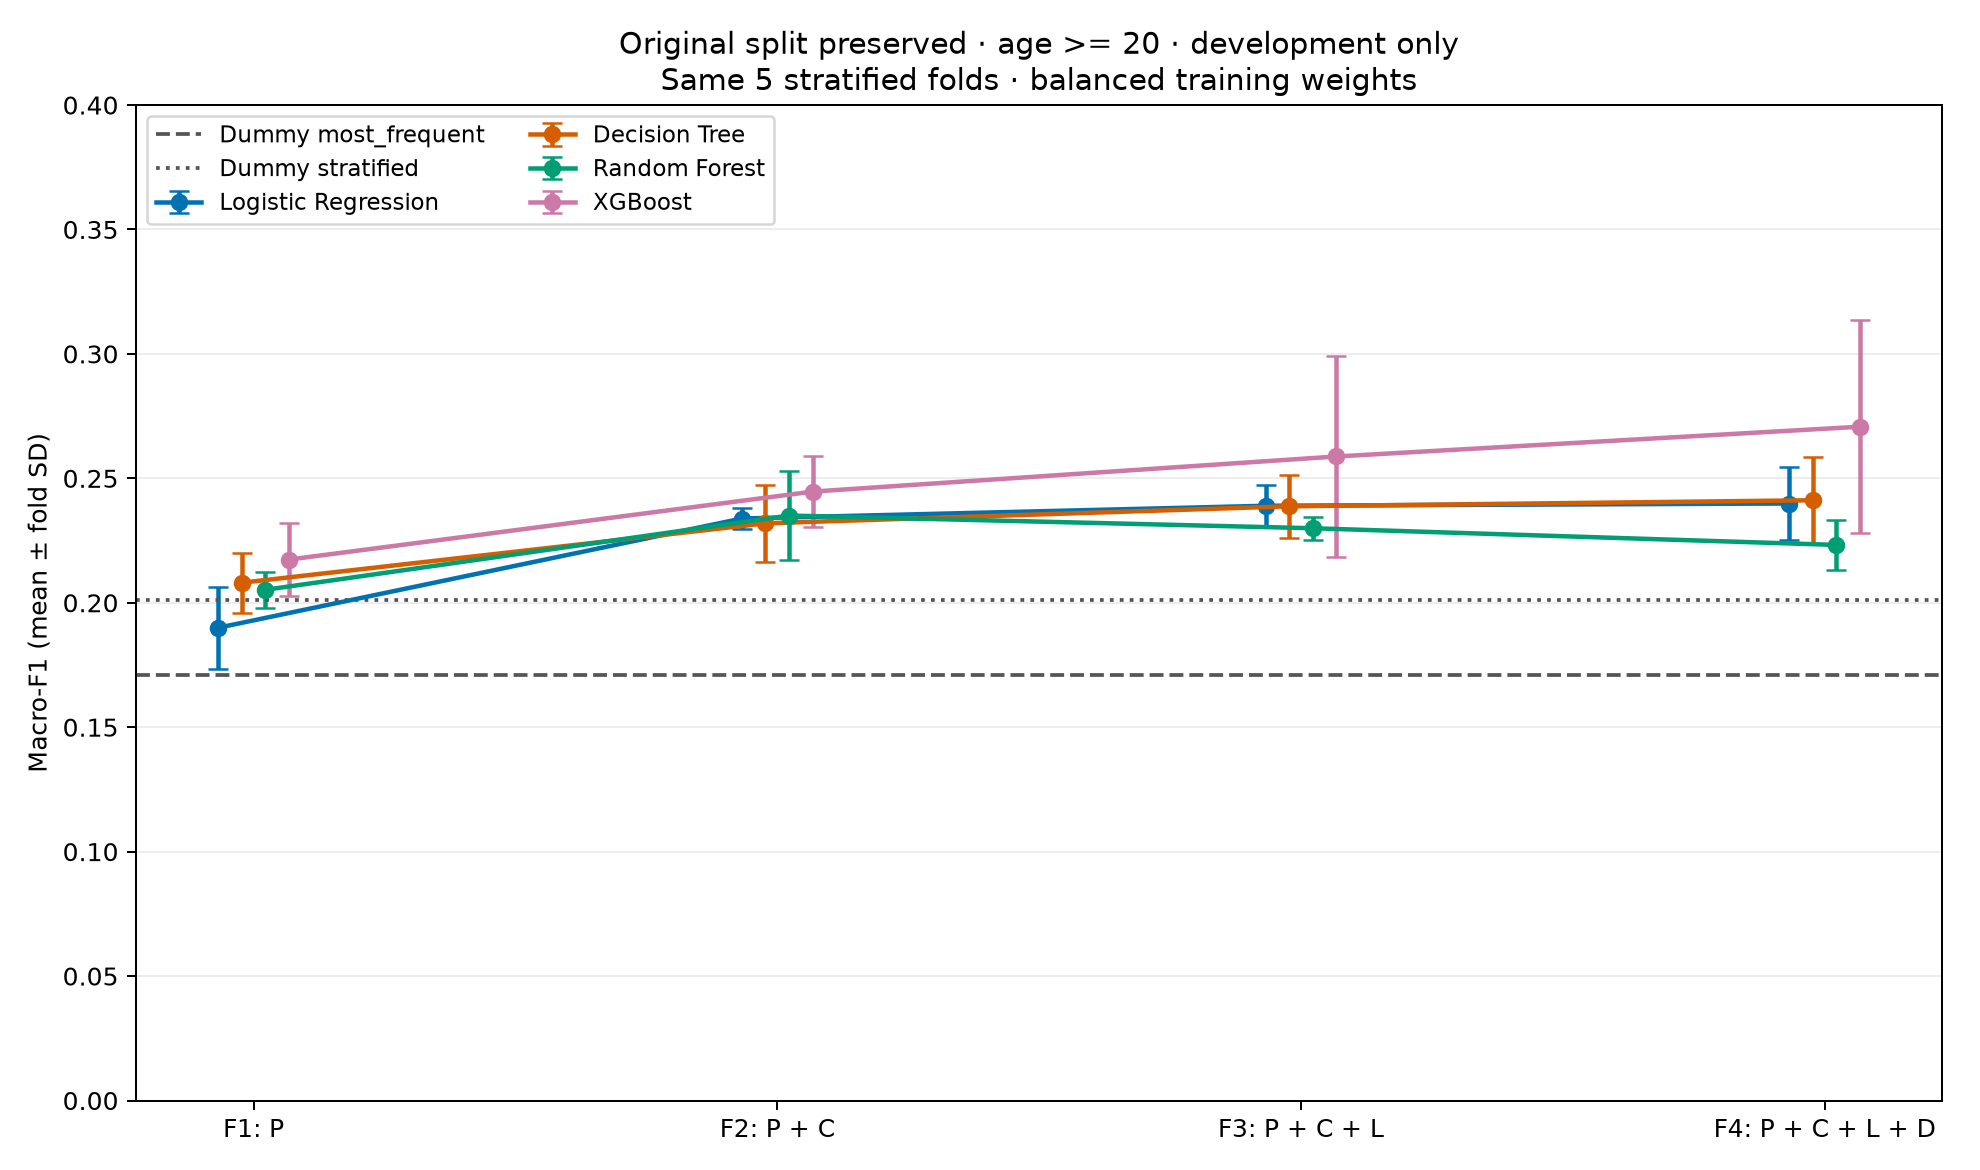
\includegraphics[width=0.9\textwidth]{figures/feature_group_comparison_final_protocol.png}
\label{fig:ablation-comparison}
\end{figure}

\subsection{Phân tích khoa học}
Từ kết quả Bảng \ref{tab:ablation-results}, một số phát hiện then chốt được rút ra:
\begin{enumerate}
    \item \textbf{Đóng góp vượt bậc của nhóm Cận lâm sàng ($F_1 \to F_2$):} Việc bổ sung các chỉ số xét nghiệm máu (HbA1c, Cholesterol, Albumin, Creatinine) tạo ra bước nhảy vọt lớn nhất về hiệu năng đối với tất cả các mô hình. Macro-F1 của Hồi quy Logistic tăng từ 0.1899 lên 0.2338 (+23.1\%), Random Forest tăng từ 0.2052 lên 0.2350 (+14.5\%), và XGBoost tăng từ 0.2173 lên 0.2447 (+12.6\%). Điều này xác nhận giả thuyết y sinh rằng các rối loạn chuyển hóa toàn thân và phản ứng viêm vi thể có mối liên kết chặt chẽ với các biểu hiện trầm cảm.
    \item \textbf{Đóng góp của nhóm Lối sống và Nhân khẩu học ($F_3, F_4$):} Nhóm đặc trưng lối sống (giấc ngủ, vận động, thuốc lá, rượu bia) và nhân khẩu học (tuổi, giới tính, học vấn, nghèo đói) tiếp tục cải thiện hiệu năng của XGBoost (từ 0.2447 lên 0.2707). Tuy nhiên, đối với Random Forest mặc định, việc tăng từ 19 lên 34 đặc trưng khiến Macro-F1 giảm nhẹ (từ 0.2350 xuống 0.2232), do thuật toán lấy mẫu ngẫu nhiên $\sqrt{d}$ đặc trưng bị phân tán bởi các biến có độ tương quan yếu. Điều này đặt ra yêu cầu cấp thiết phải thực hiện tinh chỉnh siêu tham số (Hyperparameter Tuning).
    \item \textbf{Sự khác biệt giữa Weighted-F1 và Macro-F1:} Weighted-F1 luôn đạt giá trị rất cao (từ 0.55 đến 0.67) do bị chi phối bởi lớp đa số $C_0$ (chiếm 75\%). Ngược lại, Macro-F1 chỉ dao động quanh mức 0.20 -- 0.27, phản ánh chính xác khó khăn thực sự của mô hình trong việc nhận diện các lớp thiểu số $C_2, C_3, C_4$.
\end{enumerate}

\section{Tinh chỉnh siêu tham số và Mô hình học kết hợp}
\label{sec:tuning-va-ensemble}

\subsection{Tinh chỉnh Nested Cross-Validation}
Để lựa chọn cấu hình mô hình tối ưu một cách khách quan nhất và ngăn ngừa hiện tượng quá lạc quan trong đánh giá (optimistic bias), nghiên cứu áp dụng quy trình kiểm định lồng nhau (Nested CV) \cite{varma2006bias}:
\begin{itemize}
    \item \textbf{Outer CV (5 folds):} Đánh giá hiệu năng tổng quát hóa khách quan.
    \item \textbf{Inner CV (3 folds trên Outer Training):} Thực hiện \texttt{RandomizedSearchCV} với 12 cấu hình siêu tham số ngẫu nhiên cho mỗi ứng viên trên độ đo Macro-F1.
\end{itemize}

Bốn ứng viên được đưa vào Nested Tuning gồm: \texttt{LR/F4}, \texttt{RF/F4}, \texttt{XGB/F3} và \texttt{XGB/F4}. Kết quả Nested CV (trích xuất từ \texttt{results/nested\_cv\_tuning\_report.md}):
\begin{itemize}
    \item \texttt{LR/F4}: Macro-F1 outer đạt $0.2407 \pm 0.0173$.
    \item \texttt{XGB/F3}: Macro-F1 outer đạt $0.2516 \pm 0.0267$.
    \item \texttt{XGB/F4}: Macro-F1 outer đạt $0.2621 \pm 0.0353$.
    \item \textbf{\texttt{RF/F4} (Dẫn đầu):} Macro-F1 outer đạt \textbf{0.2755 $\pm$ 0.0270} (tăng +0.0523 so với baseline RF chưa tinh chỉnh).
\end{itemize}

Bộ siêu tham số tối ưu của Random Forest trên toàn bộ tập Development: \texttt{n\_estimators = 150}, \texttt{max\_depth = 8}, \texttt{max\_features = 0.5}, \texttt{min\_samples\_split = 10}, \texttt{min\_samples\_leaf = 8}, \texttt{class\_weight = 'balanced\_subsample'}, \texttt{criterion = 'gini'}. Cấu hình này được khóa chính thức thành \textbf{Frozen Random Forest Spec} trong file cấu hình \texttt{artifacts/final\_model\_spec.json}.

\subsection{Thực nghiệm Mô hình học kết hợp (Ensemble Study)}
Nghiên cứu tiếp tục kiểm tra xem liệu việc kết hợp các mô hình (Soft Voting và Stacking) có mang lại lợi ích thực sự so với mô hình Random Forest đơn nhất hay không. Kết quả từ \texttt{results/tables/ensemble\_results.csv}:
\begin{itemize}
    \item \texttt{Frozen Random Forest (Single)}: Macro-F1 = \textbf{0.2741 $\pm$ 0.0252}, Balanced Accuracy = \textbf{0.3015 $\pm$ 0.0294}.
    \item \texttt{Soft Voting (RF + XGBoost)}: Macro-F1 = 0.2748 $\pm$ 0.0248 (chỉ tăng không đáng kể +0.0007).
    \item \texttt{Stacking Classifier (Meta-LR)}: Macro-F1 = 0.2585 $\pm$ 0.0226 (suy giảm -0.0156).
\end{itemize}

Theo quy tắc ra quyết định thận trọng (Conservative Selection Rule) đã cam kết trong đề tài: \textit{Một mô hình phức tạp hơn chỉ được chấp nhận nếu cải thiện Macro-F1 ít nhất +0.01 và thắng ít nhất 4/5 folds}. Soft Voting và Stacking đều không thỏa mãn tiêu chí này. Do đó, nghiên cứu quyết định giữ nguyên \textbf{Random Forest đã tinh chỉnh làm mô hình chuẩn tắc duy nhất}, đảm bảo sự tinh gọn và khả năng kiểm soát thuật toán cao nhất.

\section{Phân tích độ chi tiết nhãn mục tiêu ($T_2 \to T_5$)}
\label{sec:target-granularity}

\subsection{Mục tiêu và kết quả thực nghiệm}
Đây là một trong những phát hiện phương pháp luận trọng tâm nhất của đề tài, nhằm giải quyết câu hỏi \textbf{RQ2}: Lượng hóa quy luật suy giảm hiệu năng khi bài toán chuyển đổi từ phân loại nhị phân thô ($T_2$) sang các mức độ chi tiết ($T_3, T_4, T_5$) trên cùng một mô hình Frozen Random Forest và không gian đặc trưng $F_4$ ($N = 4.045$).

Kết quả thực nghiệm out-of-fold được đối chiếu từ \texttt{results/final\_report\_granularity.md} và trình bày trong Bảng \ref{tab:granularity-results}. Hình \ref{fig:granularity-curves} minh họa trực quan sự suy giảm này.

\begin{table}{Hiệu năng mô hình theo độ chi tiết nhãn mục tiêu ($T_2 \to T_5$) trên Legacy Development}
\centering
\label{tab:granularity-results}
\begin{tabular}{l c c c c c}
\toprule
\textbf{Mục tiêu} & \textbf{Số lớp ($K$)} & \textbf{Macro-F1 (Mean $\pm$ SD)} & \textbf{Balanced Acc} & \textbf{Accuracy} & \textbf{Class MAE} \\
\midrule
$T_2$ (Nhị phân)      & 2 & \textbf{0.6639 $\pm$ 0.0178} & \textbf{0.6974 $\pm$ 0.0185} & 73.57\% & 0.2643 \\
$T_3$ (3 mức gộp)     & 3 & \textbf{0.4354 $\pm$ 0.0075} & \textbf{0.4667 $\pm$ 0.0101} & 64.10\% & 0.4638 \\
$T_4$ (4 mức)         & 4 & \textbf{0.3380 $\pm$ 0.0156} & \textbf{0.3602 $\pm$ 0.0162} & 58.22\% & 0.6386 \\
$T_5$ (5 mức lâm sàng)& 5 & \textbf{0.2630 $\pm$ 0.0185} & \textbf{0.2874 $\pm$ 0.0179} & 53.15\% & 0.8124 \\
\bottomrule
\end{tabular}
\end{table}

\begin{figure}{Đồ thị thể hiện sự suy giảm nghiêm trọng của Macro-F1 và Balanced Accuracy từ $T_2$ đến $T_5$}
\centering
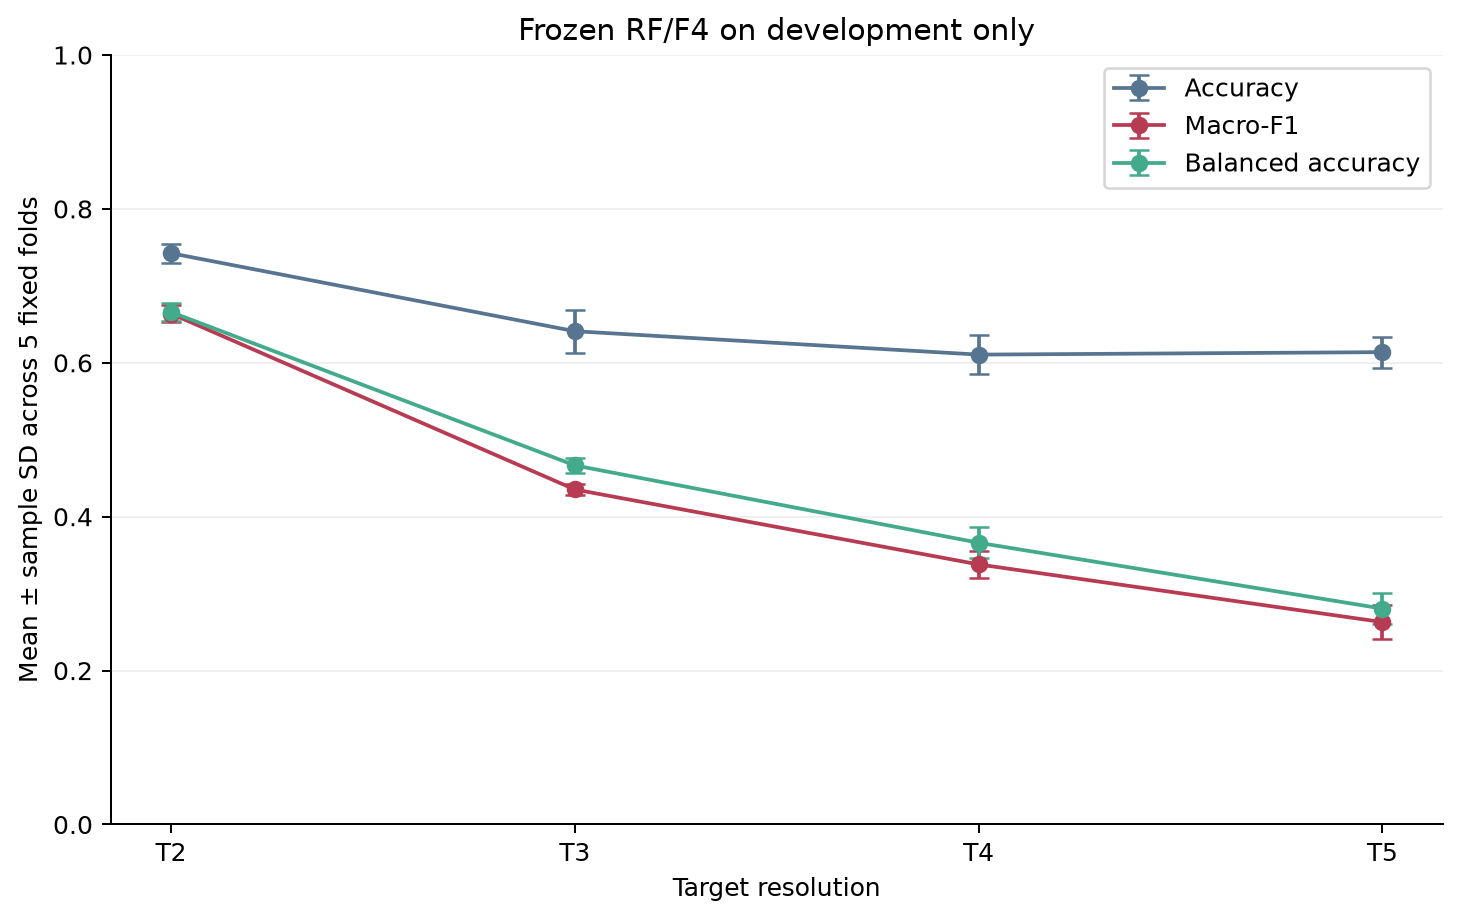
\includegraphics[width=0.85\textwidth]{figures/granularity_performance.png}
\label{fig:granularity-curves}
\end{figure}

\subsection{Phân tích nguyên nhân suy giảm và vị trí điểm nghẽn}
Từ Bảng \ref{tab:granularity-results}, sự sụt giảm hiệu năng giữa các bước chuyển đổi được lượng hóa:
\begin{itemize}
    \item \textbf{Bước chuyển $T_2 \to T_3$:} Macro-F1 sụt giảm tới \textbf{-0.2285} (từ 0.6639 xuống 0.4354, tương đương giảm 34.4\%). Đây là bước sụt giảm lớn nhất trong toàn bộ chuỗi thực nghiệm!
    \item \textbf{Bước chuyển $T_3 \to T_4$:} Macro-F1 giảm \textbf{-0.0974} (từ 0.4354 xuống 0.3380).
    \item \textbf{Bước chuyển $T_4 \to T_5$:} Macro-F1 giảm \textbf{-0.0750} (từ 0.3380 xuống 0.2630).
\end{itemize}

\textbf{Tại sao bước chuyển $T_2 \to T_3$ lại gây suy giảm mạnh nhất?}  
Trong nhiệm vụ nhị phân $T_2$, toàn bộ các đối tượng có triệu chứng từ nhẹ đến nặng ($s \ge 5$) được gộp chung thành một lớp dương tính. Mô hình chỉ cần phân tách giữa người hoàn toàn bình thường và người có bất kỳ dấu hiệu bất thường nào. Tuy nhiên, khi chuyển sang $T_3$, nhóm triệu chứng nhẹ ($C_1$: PHQ-9 từ 5 đến 9 điểm) bị tách ra thành một lớp riêng biệt nằm kẹp giữa $C_0$ và $C_2^+$. 

Phân tích ma trận nhầm lẫn của $T_3$ (Hình \ref{fig:granularity-t3-cm}) cho thấy: Lớp $C_1$ có tới 436/638 mẫu (68.3\%) bị mô hình nhầm lẫn thành $C_0$, và 98/638 mẫu (15.4\%) bị nhầm thành $C_2^+$. Độ nhạy của lớp $C_1$ chỉ đạt vỏn vẹn \textbf{16.29\%}!

\begin{figure}{Ma trận nhầm lẫn Out-of-fold của nhiệm vụ 3 lớp $T_3$, chỉ ra điểm nghẽn nghiêm trọng tại lớp $C_1$}
\centering
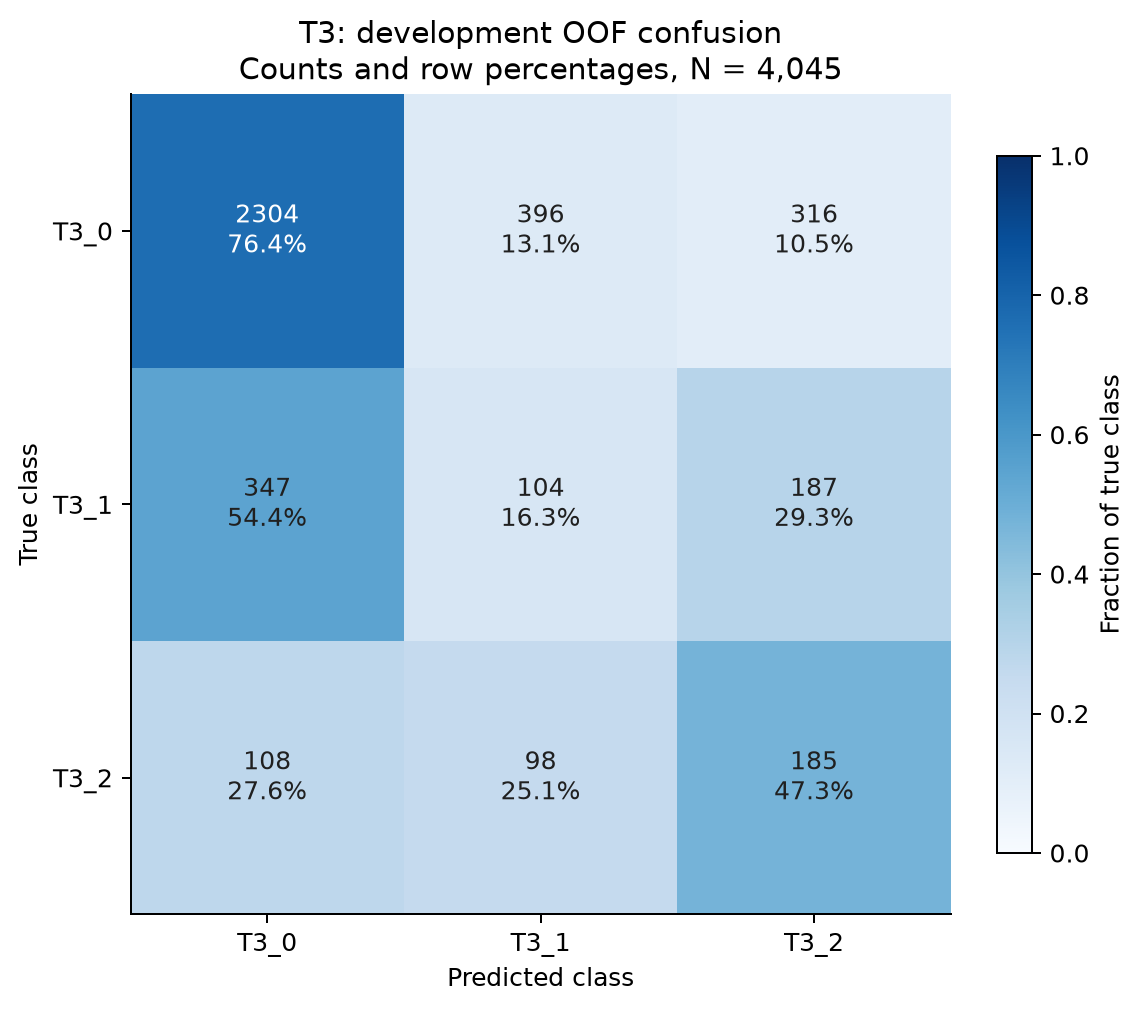
\includegraphics[width=0.65\textwidth]{figures/granularity_T3_confusion.png}
\label{fig:granularity-t3-cm}
\end{figure}

Phân tích thành phần chính (PCA) trên không gian đặc trưng sinh lý (Hình \ref{fig:overlap-pca}) khẳng định một sự thật khách quan: Các điểm dữ liệu của $C_0$ và $C_1$ chồng lấn gần như hoàn toàn lên nhau. Sự khác biệt về huyết áp, đường huyết hay mỡ máu giữa một người có 4 điểm PHQ-9 (xếp vào $C_0$) và một người có 5 điểm PHQ-9 (xếp vào $C_1$) là cực kỳ mong manh và không mang tính phân tách thống kê rõ rệt.

\begin{figure}{Trực quan hóa không gian đặc trưng bằng PCA: Sự chồng lấn phân phối sinh lý dày đặc giữa các mức độ triệu chứng}
\centering
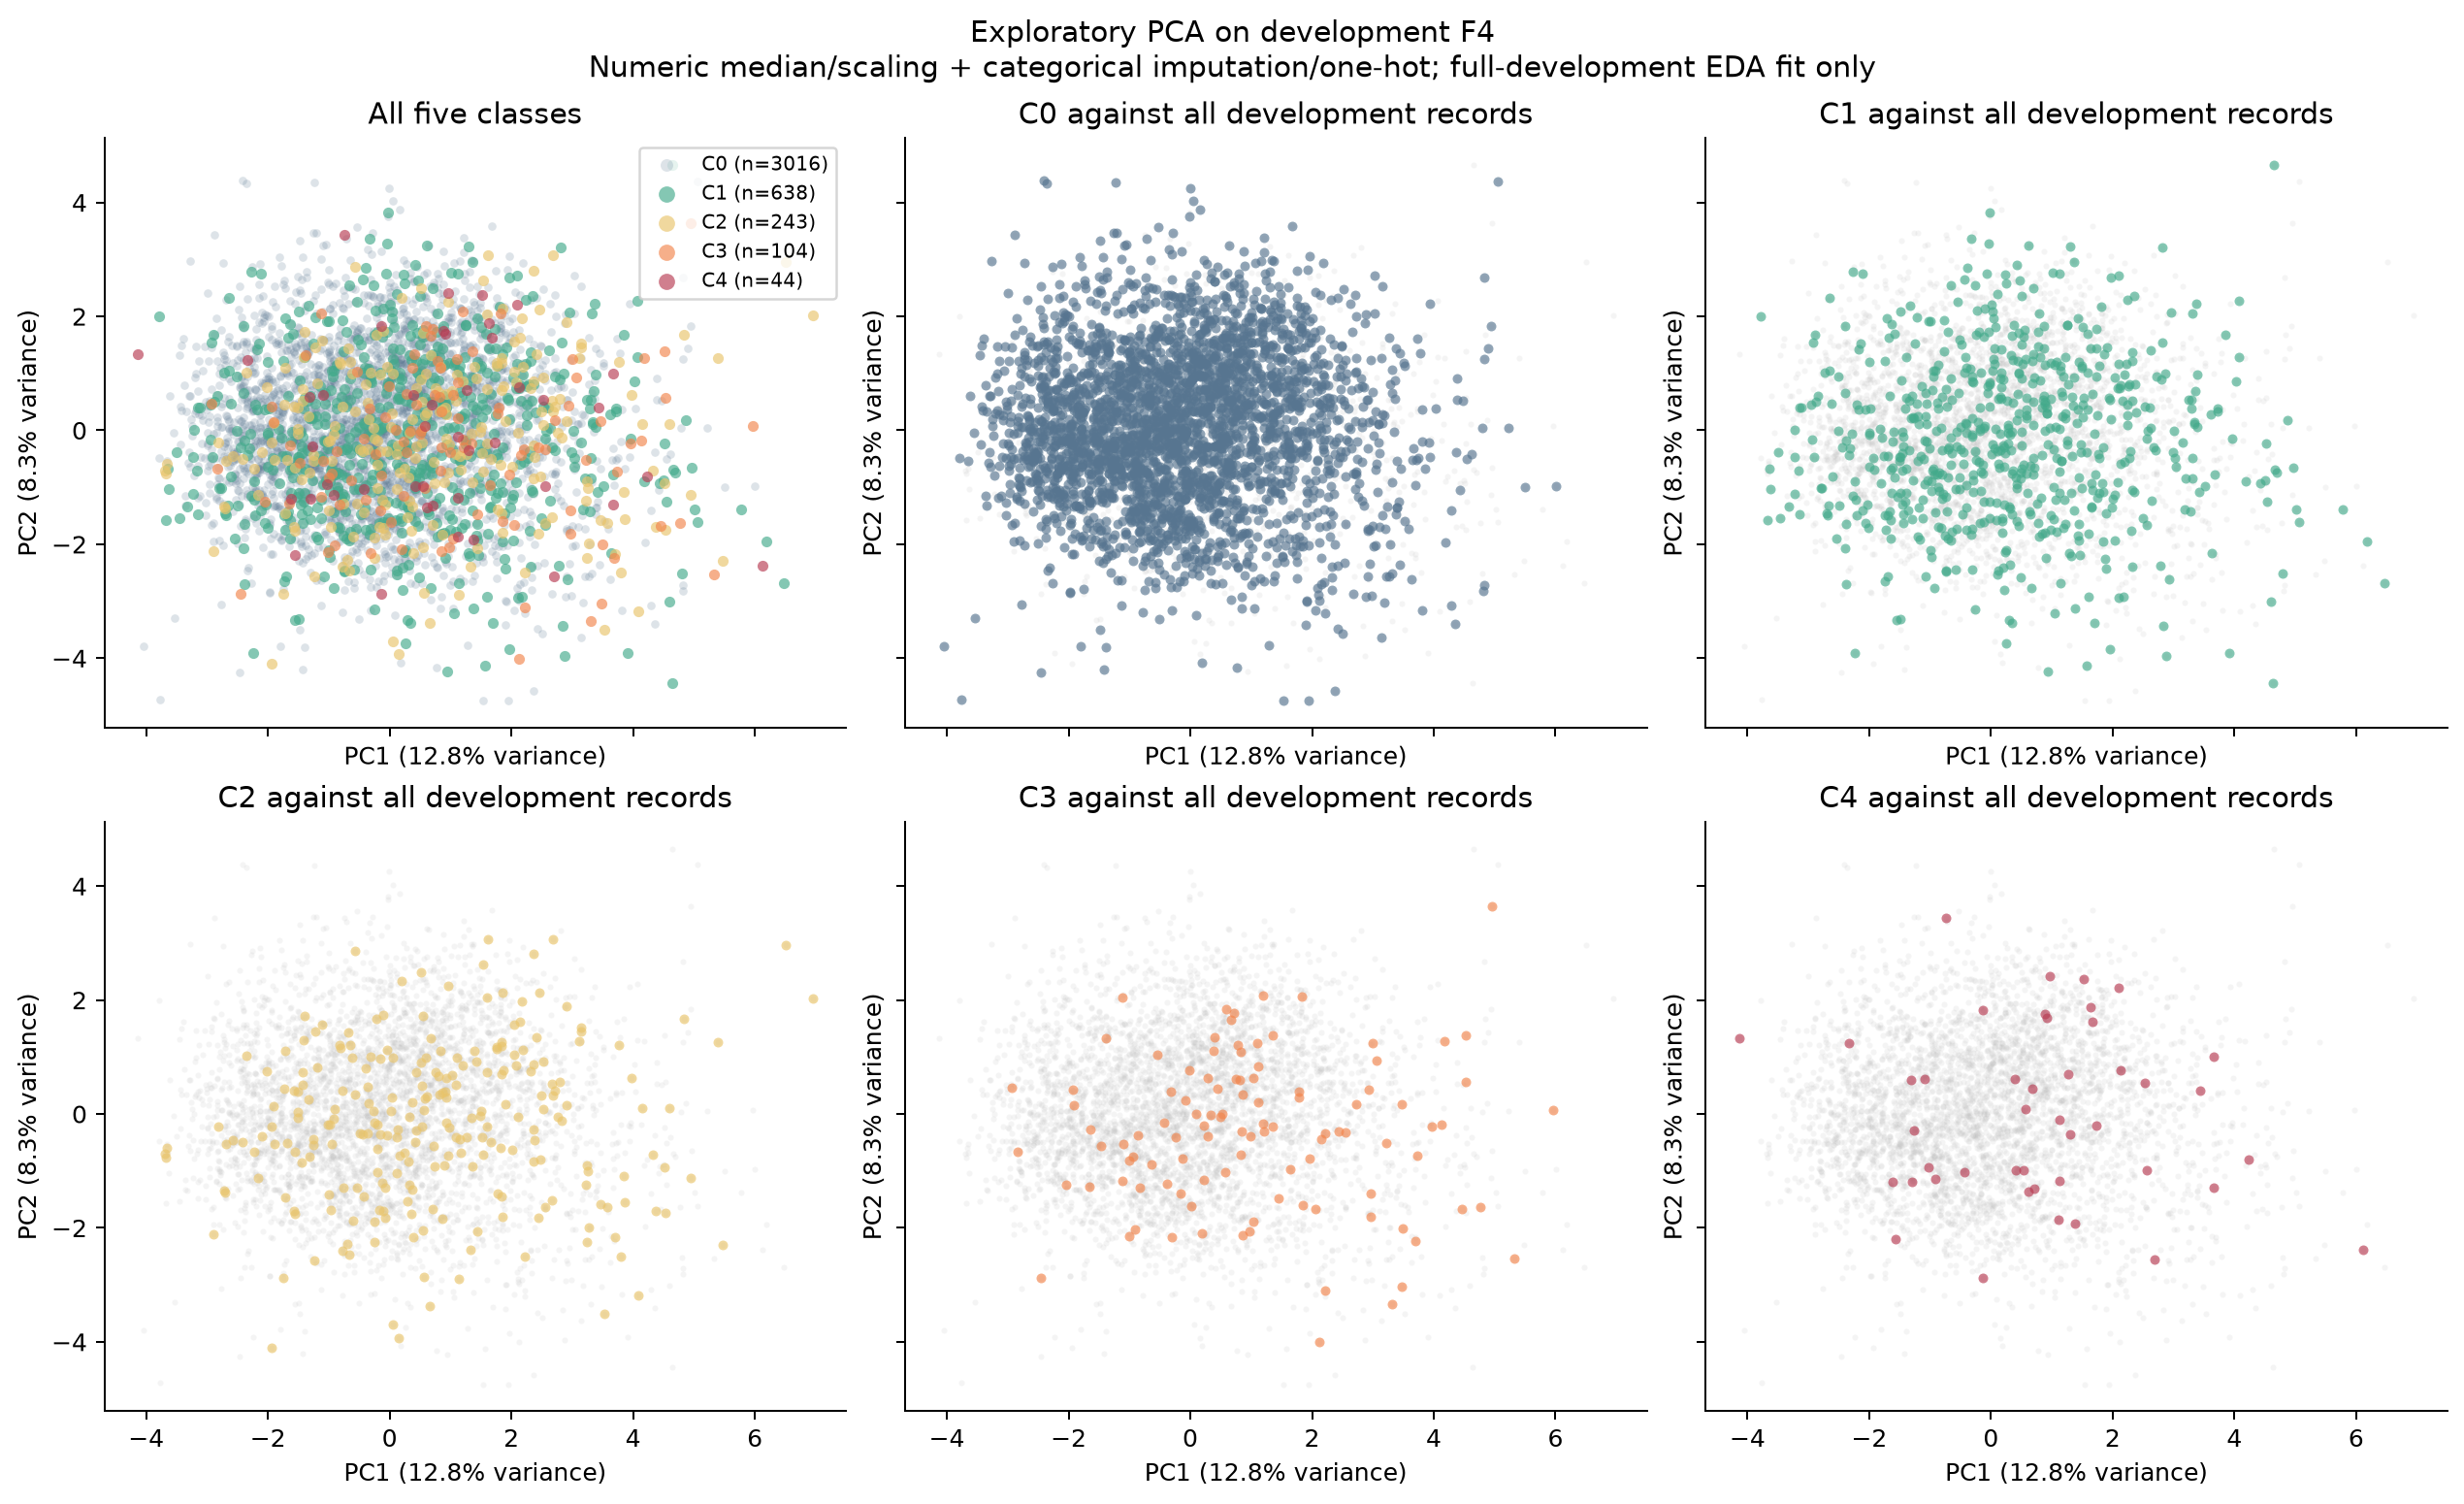
\includegraphics[width=0.75\textwidth]{figures/overlap_pca_C0_C4.png}
\label{fig:overlap-pca}
\end{figure}

\section{Thực nghiệm Tổng quát hóa trên Multi-Cycle Cohort}
\label{sec:thuc-nghiem-multicycle}

Để trả lời câu hỏi nghiên cứu \textbf{RQ3}, framework DepSev-ML được mở rộng đánh giá trên tập dữ liệu đa chu kỳ chính thức với không gian đặc trưng hài hòa $F_{4\_\text{common31}}$ gồm 31 biến số. Bốn nhánh thực nghiệm có kiểm soát được thiết kế:
\begin{itemize}
    \item \textbf{Branch A (Single-cycle 2013--2014, $N = 5.054$):} Đóng vai trò là đối chứng chu kỳ đơn hợp lệ trong cùng không gian đặc trưng Common31.
    \item \textbf{Branch B (Pooled Multi-cycle 2011--2016, $N = 14.581$):} Gộp toàn bộ 3 chu kỳ để tăng cỡ mẫu lên gấp gần 3 lần.
    \item \textbf{Branch C (Matched-N, $N = 5.054$):} Lấy mẫu ngẫu nhiên từ tập Pooled sao cho cỡ mẫu đúng bằng Branch A nhằm cô lập tác động của quy mô mẫu khỏi thành phần chu kỳ.
    \item \textbf{Branch D (Temporal Evaluation):} Huấn luyện trên hai chu kỳ quá khứ 2011--2014 ($N = 9.693$), kiểm tra độc lập trên chu kỳ tương lai 2015--2016 ($N = 4.888$).
\end{itemize}

Kết quả thực nghiệm trên nhiệm vụ 5 lớp $T_5$ (trích xuất từ \texttt{results/final\_report\_integrated.md}):
\begin{itemize}
    \item \textbf{Macro-F1 không tăng khi gộp dữ liệu:} Branch A đạt Macro-F1 = \textbf{0.2634 $\pm$ 0.0152}, trong khi Branch B đạt Macro-F1 = \textbf{0.2619 $\pm$ 0.0098}. Sự khác biệt là hoàn toàn không đáng kể (-0.0015).
    \item \textbf{Balanced Accuracy cải thiện nhẹ:} Tăng từ \textbf{0.2841 $\pm$ 0.0142} (Branch A) lên \textbf{0.3076 $\pm$ 0.0118} (Branch B).
    \item \textbf{Recall của các lớp nặng hiếm mẫu ($C_3, C_4$) được cải thiện:} Khi số lượng mẫu $C_4$ trong tập huấn luyện tăng từ 55 lên 167 mẫu, độ nhạy Recall $C_4$ tăng từ 10.91\% lên 17.37\%. Tuy nhiên, độ chính xác dự đoán (Precision) của $C_4$ vẫn ở mức rất thấp (khoảng 3--5\%), do đó điểm F1 của các lớp này hầu như không thay đổi và không kéo tăng được Macro-F1 tổng thể.
    \item \textbf{Kiểm định thời gian (Branch D):} Trên tập dữ liệu độc lập 2015--2016 ($N = 4.888$), mô hình duy trì Macro-F1 = \textbf{0.2584} và Balanced Accuracy = \textbf{0.3012}, chứng minh mô hình không bị quá khớp theo thời gian nhưng trần hiệu năng phân loại đa mức vẫn tồn tại bất biến.

\end{itemize}

\textbf{Kết luận RQ3:} Việc mở rộng cỡ mẫu đa chu kỳ giúp mô hình ước lượng phân phối của các lớp hiếm ổn định hơn (tăng nhẹ Balanced Accuracy và Recall lớp nặng), nhưng \textbf{không thể phá vỡ trần suy giảm hiệu năng của bài toán phân loại đa mức chi tiết} nếu không gian đặc trưng sinh lý vẫn có độ chồng lấn cao.

\section{Thực nghiệm $T_3$ – So sánh Phân loại Phẳng và Phân cấp Cứng}
\label{sec:thuc-nghiem-t3-hard}

Để tìm giải pháp kiến trúc khắc phục hiện tượng suy giảm hiệu năng trên không gian 3 lớp $T_3$ ($C_0, C_1, C_2^+$), nghiên cứu triển khai nhóm thực nghiệm Phân loại phân cấp hai tầng cứng ($E_1 \to E_3b$) đối chứng với mô hình Phân loại phẳng $E_0$ (Random Forest phẳng).

Các mô hình được đánh giá bao gồm:
\begin{itemize}
    \item \texttt{E0\_Flat\_RF}: Random Forest phân loại trực tiếp 3 lớp.
    \item \texttt{E1\_Hard\_RF\_RF}: Hard Hierarchical RF (Tầng 1) + RF (Tầng 2), ngưỡng cắt $\tau_1 = \tau_2 = 0.5$.
    \item \texttt{E2\_Hard\_Tuned}: Hard Hierarchical RF--RF với ngưỡng cắt được tối ưu hóa qua lưới bằng Inner CV ($\tau_1 = 0.40, \tau_2 = 0.50$).
    \item \texttt{E3a\_Hard\_RF\_LR}: Hard Hierarchical RF (Tầng 1) + Hồi quy Logistic cân bằng (Tầng 2).
    \item \texttt{E3b\_Hard\_RF\_XGB}: Hard Hierarchical RF (Tầng 1) + XGBoost cân bằng (Tầng 2).
\end{itemize}

Kết quả thực nghiệm out-of-fold trên Legacy Development Cohort ($N = 4.045$) được tổng hợp trong Bảng \ref{tab:hard-hierarchical-results}.

\begin{table}{So sánh hiệu năng giữa Flat Classification và Hard Hierarchical trên nhiệm vụ $T_3$}
\centering
\label{tab:hard-hierarchical-results}
\begin{tabular}{l c c c c c c}
\toprule
\textbf{Mô hình} & \textbf{Macro-F1} & \textbf{BalAcc} & \textbf{Accuracy} & \textbf{Recall $C_1$} & \textbf{Recall $C_2^+$} & \textbf{Bỏ sót $C_2^+ \to C_0$} \\
\midrule
$E_0$ (Flat RF)       & 0.4354 $\pm$ 0.0075 & 0.4667 & 64.10\% & 16.29\% & 47.32\% & 108 ca \\
$E_1$ (Hard RF--RF)   & 0.4550 $\pm$ 0.0056 & 0.4745 & 68.08\% & 16.46\% & 43.74\% & 120 ca \\
$E_2$ (Hard Tuned)    & \textbf{0.4586 $\pm$ 0.0124} & 0.4902 & 65.32\% & \textbf{25.69\%} & 39.63\% & 95 ca \\
$E_3a$ (Hard RF--LR)  & 0.4567 $\pm$ 0.0271 & \textbf{0.4964} & \textbf{68.43\%} & 11.75\% & \textbf{55.00\%} & 120 ca \\
$E_3b$ (Hard RF--XGB) & 0.4575 $\pm$ 0.0182 & 0.4856 & 68.23\% & 16.77\% & 44.76\% & 120 ca \\
\bottomrule
\end{tabular}
\end{table}

\textbf{Phát hiện về Error Propagation của Hard Routing:}
Mặc dù các mô hình phân cấp $E_1, E_2, E_3a$ đều cải thiện được Macro-F1 so với mô hình phẳng $E_0$ (tăng từ 0.4354 lên 0.4550 -- 0.4586), phân tích luồng dữ liệu chỉ ra một khiếm khuyết lâm sàng nghiêm trọng:
Tại Giai đoạn 1, cổng phân loại nhị phân cứng với ngưỡng $\tau_1 = 0.5$ đã loại bỏ nhầm \textbf{120 bệnh nhân thuộc nhóm Nặng quy ước ($C_2^+$)} (chiếm tới 30.7\% tổng số 391 bệnh nhân nặng). Những bệnh nhân này bị dán nhãn ngay lập tức là $C_0$ (bình thường) và không bao giờ có cơ hội được Giai đoạn 2 xem xét. Đây là minh chứng thực nghiệm điển hình cho hiện tượng lan truyền sai số một chiều trong kiến trúc phân cấp cứng.

\section{Thực nghiệm Soft Hierarchical và Quyết định Nhạy chi phí ($E_4 \to E_6$)}
\label{sec:thuc-nghiem-soft-cost}

Để khắc phục hiện tượng tắc nghẽn của cổng cứng, nhóm thực nghiệm $E_4 \to E_6b$ được triển khai:
\begin{itemize}
    \item \texttt{$E\_4$ (Soft RF--RF)}: Tích hợp xác suất toàn phần, ra quyết định bằng Argmax.
    \item \texttt{$E\_5$ (Soft RF--LR)}: Tích hợp xác suất toàn phần với Tầng 2 là Logistic Regression, ra quyết định bằng Argmax.
    \item \texttt{$E\_6a$ (Soft RF--RF + Cost M1)}: Tối ưu hóa rủi ro Bayes với ma trận chi phí lâm sàng $M_1$.
    \item \texttt{$E\_6b$ (Soft RF--LR + Cost M1)}: Tối ưu hóa rủi ro Bayes với ma trận chi phí $M_1$.
\end{itemize}

Kết quả thực nghiệm out-of-fold trên Legacy Development Cohort ($N = 4.045$) được trình bày trong Bảng \ref{tab:soft-cost-results}. Hình \ref{fig:cost-curve} thể hiện đường cong đánh đổi chi phí khi tăng mức phạt qua các ma trận $M_0 \to M_3$.

\begin{table}{Hiệu năng mô hình Soft Hierarchical và Quyết định Nhạy chi phí ($N = 4.045$)}
\centering
\label{tab:soft-cost-results}
\begin{tabular}{l c c c c c c}
\toprule
\textbf{Mô hình} & \textbf{Macro-F1} & \textbf{BalAcc} & \textbf{Accuracy} & \textbf{Recall $C_2^+$} & \textbf{$C_2^+ \to C_0$} & \textbf{$C_0 \to C_2^+$ (FA)} \\
\midrule
$E_4$ (Soft RF--RF Argmax) & 0.4206 $\pm$ 0.0104 & 0.4309 & \textbf{73.75\%} & 30.19\% & 227 ca & \textbf{139 ca} \\
$E_5$ (Soft RF--LR Argmax) & 0.4270 $\pm$ 0.0118 & 0.4506 & 73.37\% & 39.13\% & 211 ca & 176 ca \\
$E_6a$ (Soft RF--RF + Cost M1) & 0.4535 $\pm$ 0.0149 & 0.4904 & 56.91\% & 44.25\% & 62 ca & 1.148 ca \\
$E_6b$ (Soft RF--LR + Cost M1) & \textbf{0.4521 $\pm$ 0.0190} & \textbf{0.5025} & 56.84\% & \textbf{54.23\%} & \textbf{62 ca} & 294 ca \\
\bottomrule
\end{tabular}
\end{table}

\begin{figure}{Đường cong đánh đổi giữa việc giảm số ca bỏ sót nặng ($C_2^+ \to C_0$) và sự gia tăng cảnh báo giả ($C_0 \to C_2^+$) qua các ma trận chi phí $M_0 \to M_3$}
\centering
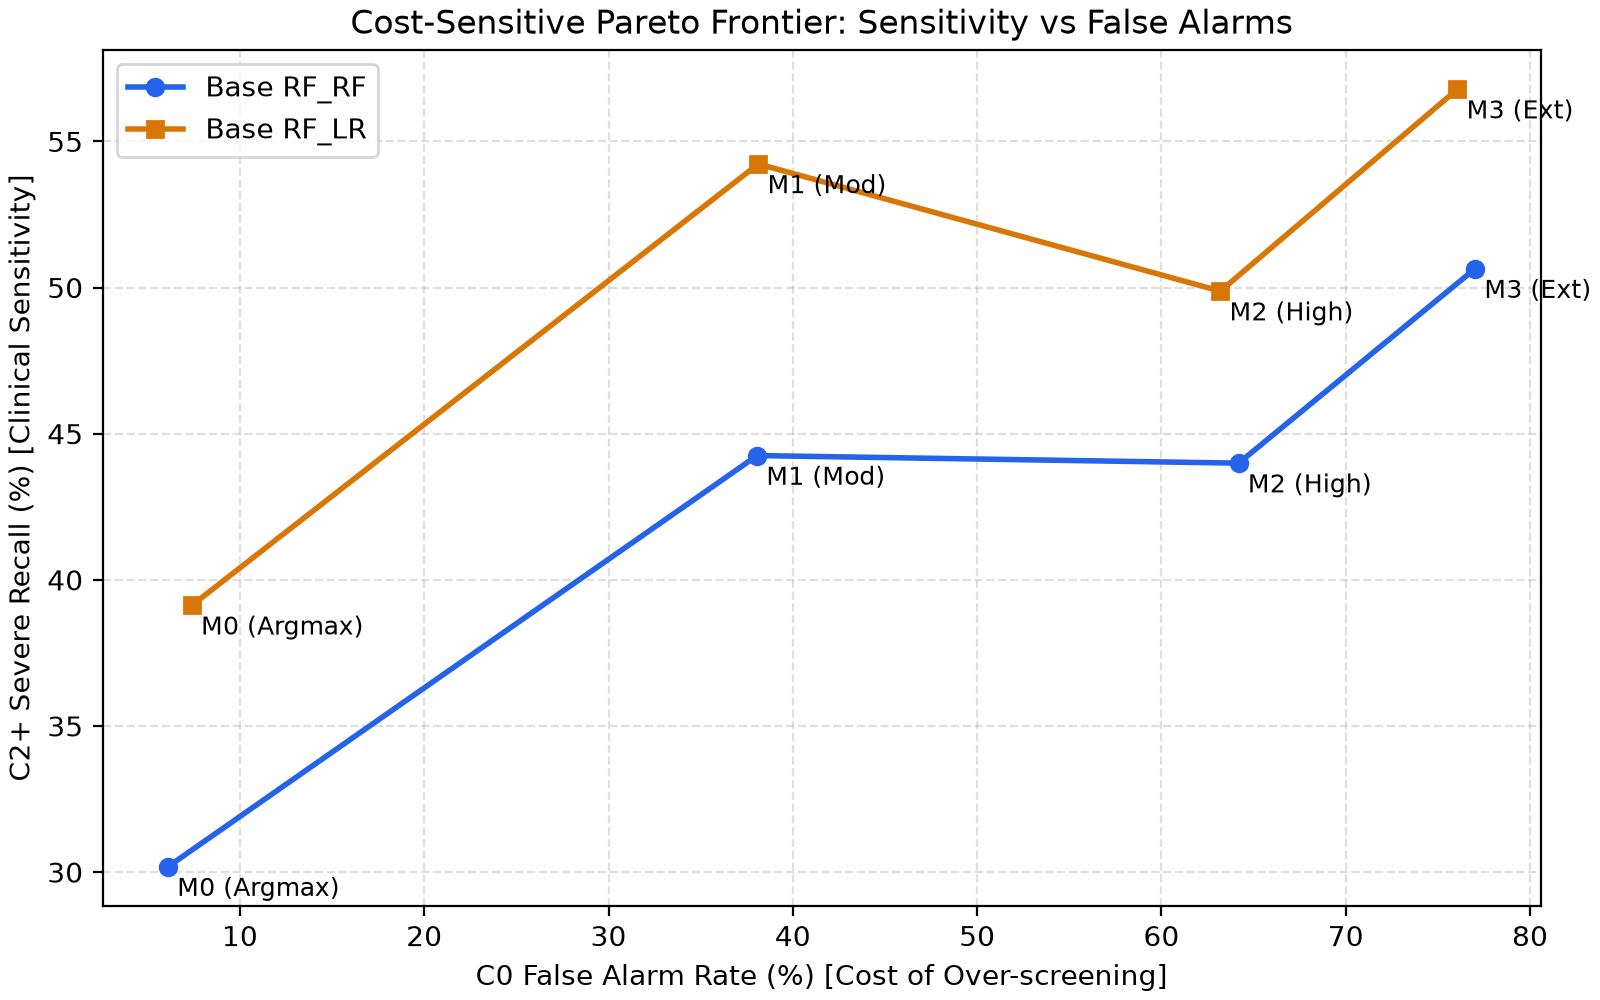
\includegraphics[width=0.85\textwidth]{figures/cost_tradeoff_curve.png}
\label{fig:cost-curve}
\end{figure}

\textbf{Phân tích khoa học:}
1. \textbf{Hạn chế của Soft Argmax ($E_4, E_5$):} Khi chỉ dùng Argmax xác suất mà không có ma trận chi phí, mô hình bị thiên lệch cực mạnh về lớp đa số $C_0$ (Recall $C_0 > 92\%$, nhưng Recall $C_1 < 5.2\%$). Số ca nặng $C_2^+$ bị bỏ sót thành $C_0$ tăng vọt lên \textbf{211 ca} ($E_5$) và \textbf{227 ca} ($E_4$).  
2. \textbf{Tác dụng giải cứu của Ma trận chi phí lâm sàng $M_1$ ($E_6b$):} Khi áp dụng quy tắc rủi ro Bayes với ma trận $M_1$, mô hình $E_6b$ đã kéo số ca bỏ sót nguy hiểm $C_2^+ \to C_0$ từ 211 ca xuống chỉ còn \textbf{62 ca} (giảm 70.6\%), đồng thời nâng Recall $C_2^+$ lên \textbf{54.23\%} và Balanced Accuracy đạt \textbf{0.5025}.
3. \textbf{Cảnh báo về sự đánh đổi khi tăng phạt cực đoan ($M_2, M_3$):} Nếu tiếp tục tăng mức phạt qua $M_2$ và $M_3$, số ca $C_2^+ \to C_0$ có thể giảm xuống 19 và 7 ca, nhưng số ca cảnh báo giả $C_0 \to C_2^+$ sẽ bùng nổ lên tới 1.906 và 2.294 ca, phá hủy hoàn toàn độ đặc hiệu của hệ thống sàng lọc. Do đó $M_1$ là điểm cân bằng tối ưu duy nhất.

\section{Thực nghiệm Phân loại Thứ bậc (Ordinal Classification -- $E_7$)}
\label{sec:thuc-nghiem-ordinal}

\subsection{Mục tiêu và các mô hình thử nghiệm}
Thực nghiệm $E_7$ nhằm trả lời câu hỏi cốt lõi: Khai thác trực tiếp thứ tự tự nhiên $C_0 \prec C_1 \prec C_2^+$ thông qua các mô hình Ordinal Classification có mang lại hiệu năng vượt trội và giải quyết được sự đánh đổi giữa các chỉ số hay không. Bốn mô hình được đánh giá:
\begin{itemize}
    \item \texttt{E7a\_Ordinal\_LogReg}: Mô hình Proportional Odds Cumulative Logit, không dùng trọng số.
    \item \texttt{E7a\_Ordinal\_LogReg\_Balanced}: Mô hình Proportional Odds với \texttt{class\_weight="balanced"}.
    \item \texttt{E7b\_CumBin\_LR}: Mô hình Frank \& Hall với bộ phân loại cơ sở là Logistic Regression.
    \item \texttt{E7b\_CumBin\_RF}: Mô hình Frank \& Hall với bộ phân loại cơ sở là Random Forest.
\end{itemize}

Kết quả thực nghiệm out-of-fold chi tiết trên Legacy Development ($N = 4.045$) được trình bày trong Bảng \ref{tab:ordinal-results}.

\begin{table}{Kết quả thực nghiệm các mô hình Ordinal Classification trên nhiệm vụ $T_3$}
\centering
\label{tab:ordinal-results}
\begin{tabular}{l c c c c c c c}
\toprule
\textbf{Mô hình} & \textbf{Macro-F1} & \textbf{BalAcc} & \textbf{Accuracy} & \textbf{Class MAE} & \textbf{QWK} & \textbf{Recall $C_1$} & \textbf{Recall $C_2^+$} \\
\midrule
$E_{7a}$ (OLR Unweighted) & 0.3846 & 0.4002 & \textbf{75.23\%} & \textbf{0.3377} & 0.2298 & 0.00\% & 22.00\% \\
$E_{7a}$ (OLR Balanced)   & \textbf{0.4518} & \textbf{0.5151} & 56.69\% & 0.5382 & 0.3398 & \textbf{32.93\%} & \textbf{60.37\%} \\
$E_{7b}$ (CumBin LR)      & 0.3761 & 0.4949 & 63.41\% & 0.5718 & 0.2958 & 0.00\% & 72.88\% \\
$E_{7b}$ (CumBin RF)      & 0.4191 & 0.4900 & 72.34\% & 0.3953 & \textbf{0.3744} & 0.16\% & 57.30\% \\
\bottomrule
\end{tabular}
\end{table}

\subsection{Phân tích hiện tượng suy biến lớp trung gian và vi phạm đơn điệu}
Thực nghiệm $E_7$ mang lại hai phát hiện khoa học đặc biệt quan trọng:

\textbf{1. Nghịch lý của Class MAE trong E7a không trọng số:}  
Mô hình \texttt{E7a} không trọng số đạt \textbf{Class MAE thấp nhất (0.3377)} và \textbf{Accuracy cao nhất (75.23\%)} trong toàn bộ 10 mô hình của dự án. Tuy nhiên, mô hình hoàn toàn không nhận diện được bất kỳ mẫu nào thuộc lớp $C_1$ (\textbf{Recall $C_1 = 0.00\%$}).  
*Giải thích:* Do hàm mất mát MAE phạt sai lệch theo khoảng cách $|y - \hat{y}|$, việc dự đoán toàn bộ về lớp đa số $C_0$ khiến 74.5\% mẫu có lỗi bằng 0, 15.8\% mẫu $C_1$ chỉ chịu lỗi bằng 1, và 9.7\% mẫu $C_2^+$ chịu lỗi bằng 2. Bộ tối ưu hóa tự nhiên triệt tiêu lớp trung gian $C_1$ để tối thiểu hóa MAE kỳ vọng. Điều này chứng minh rằng: \textbf{Chỉ dựa vào Class MAE thấp để kết luận mô hình thứ bậc tốt là một sai lầm nghiêm trọng trên dữ liệu mất cân bằng.}

\textbf{2. Sự sụp đổ của phương pháp Frank \& Hall (E7b):}  
Do hai bộ phân loại nhị phân $P(Y \ge 1)$ và $P(Y \ge 2)$ được huấn luyện độc lập, các siêu phẳng quyết định bị cắt nhau trong không gian đặc trưng. Thống kê out-of-fold ghi nhận \textbf{19.53\% số mẫu kiểm tra bị vi phạm tính đơn điệu ($q_2 > q_1$)} đối với Logistic Regression và \textbf{5.32\%} đối với Random Forest (Hình \ref{fig:monotonicity-violations}). Sau phép chiếu đẳng điệu $(q_1 + q_2)/2$, khoảng cách xác suất của lớp $C_1$ bị triệt tiêu hoàn toàn, khiến Recall $C_1$ của $E_{7b}$ rơi về 0.00\% (LR) và 0.16\% (RF), đồng thời gây ra tới \textbf{727 ca cảnh báo giả nặng ($C_0 \to C_2^+$)}.

\begin{figure}{Tỷ lệ vi phạm tính đơn điệu ($q_2 > q_1$) trên 5 folds kiểm định chéo của phương pháp Frank \& Hall ($E_7b$)}
\centering
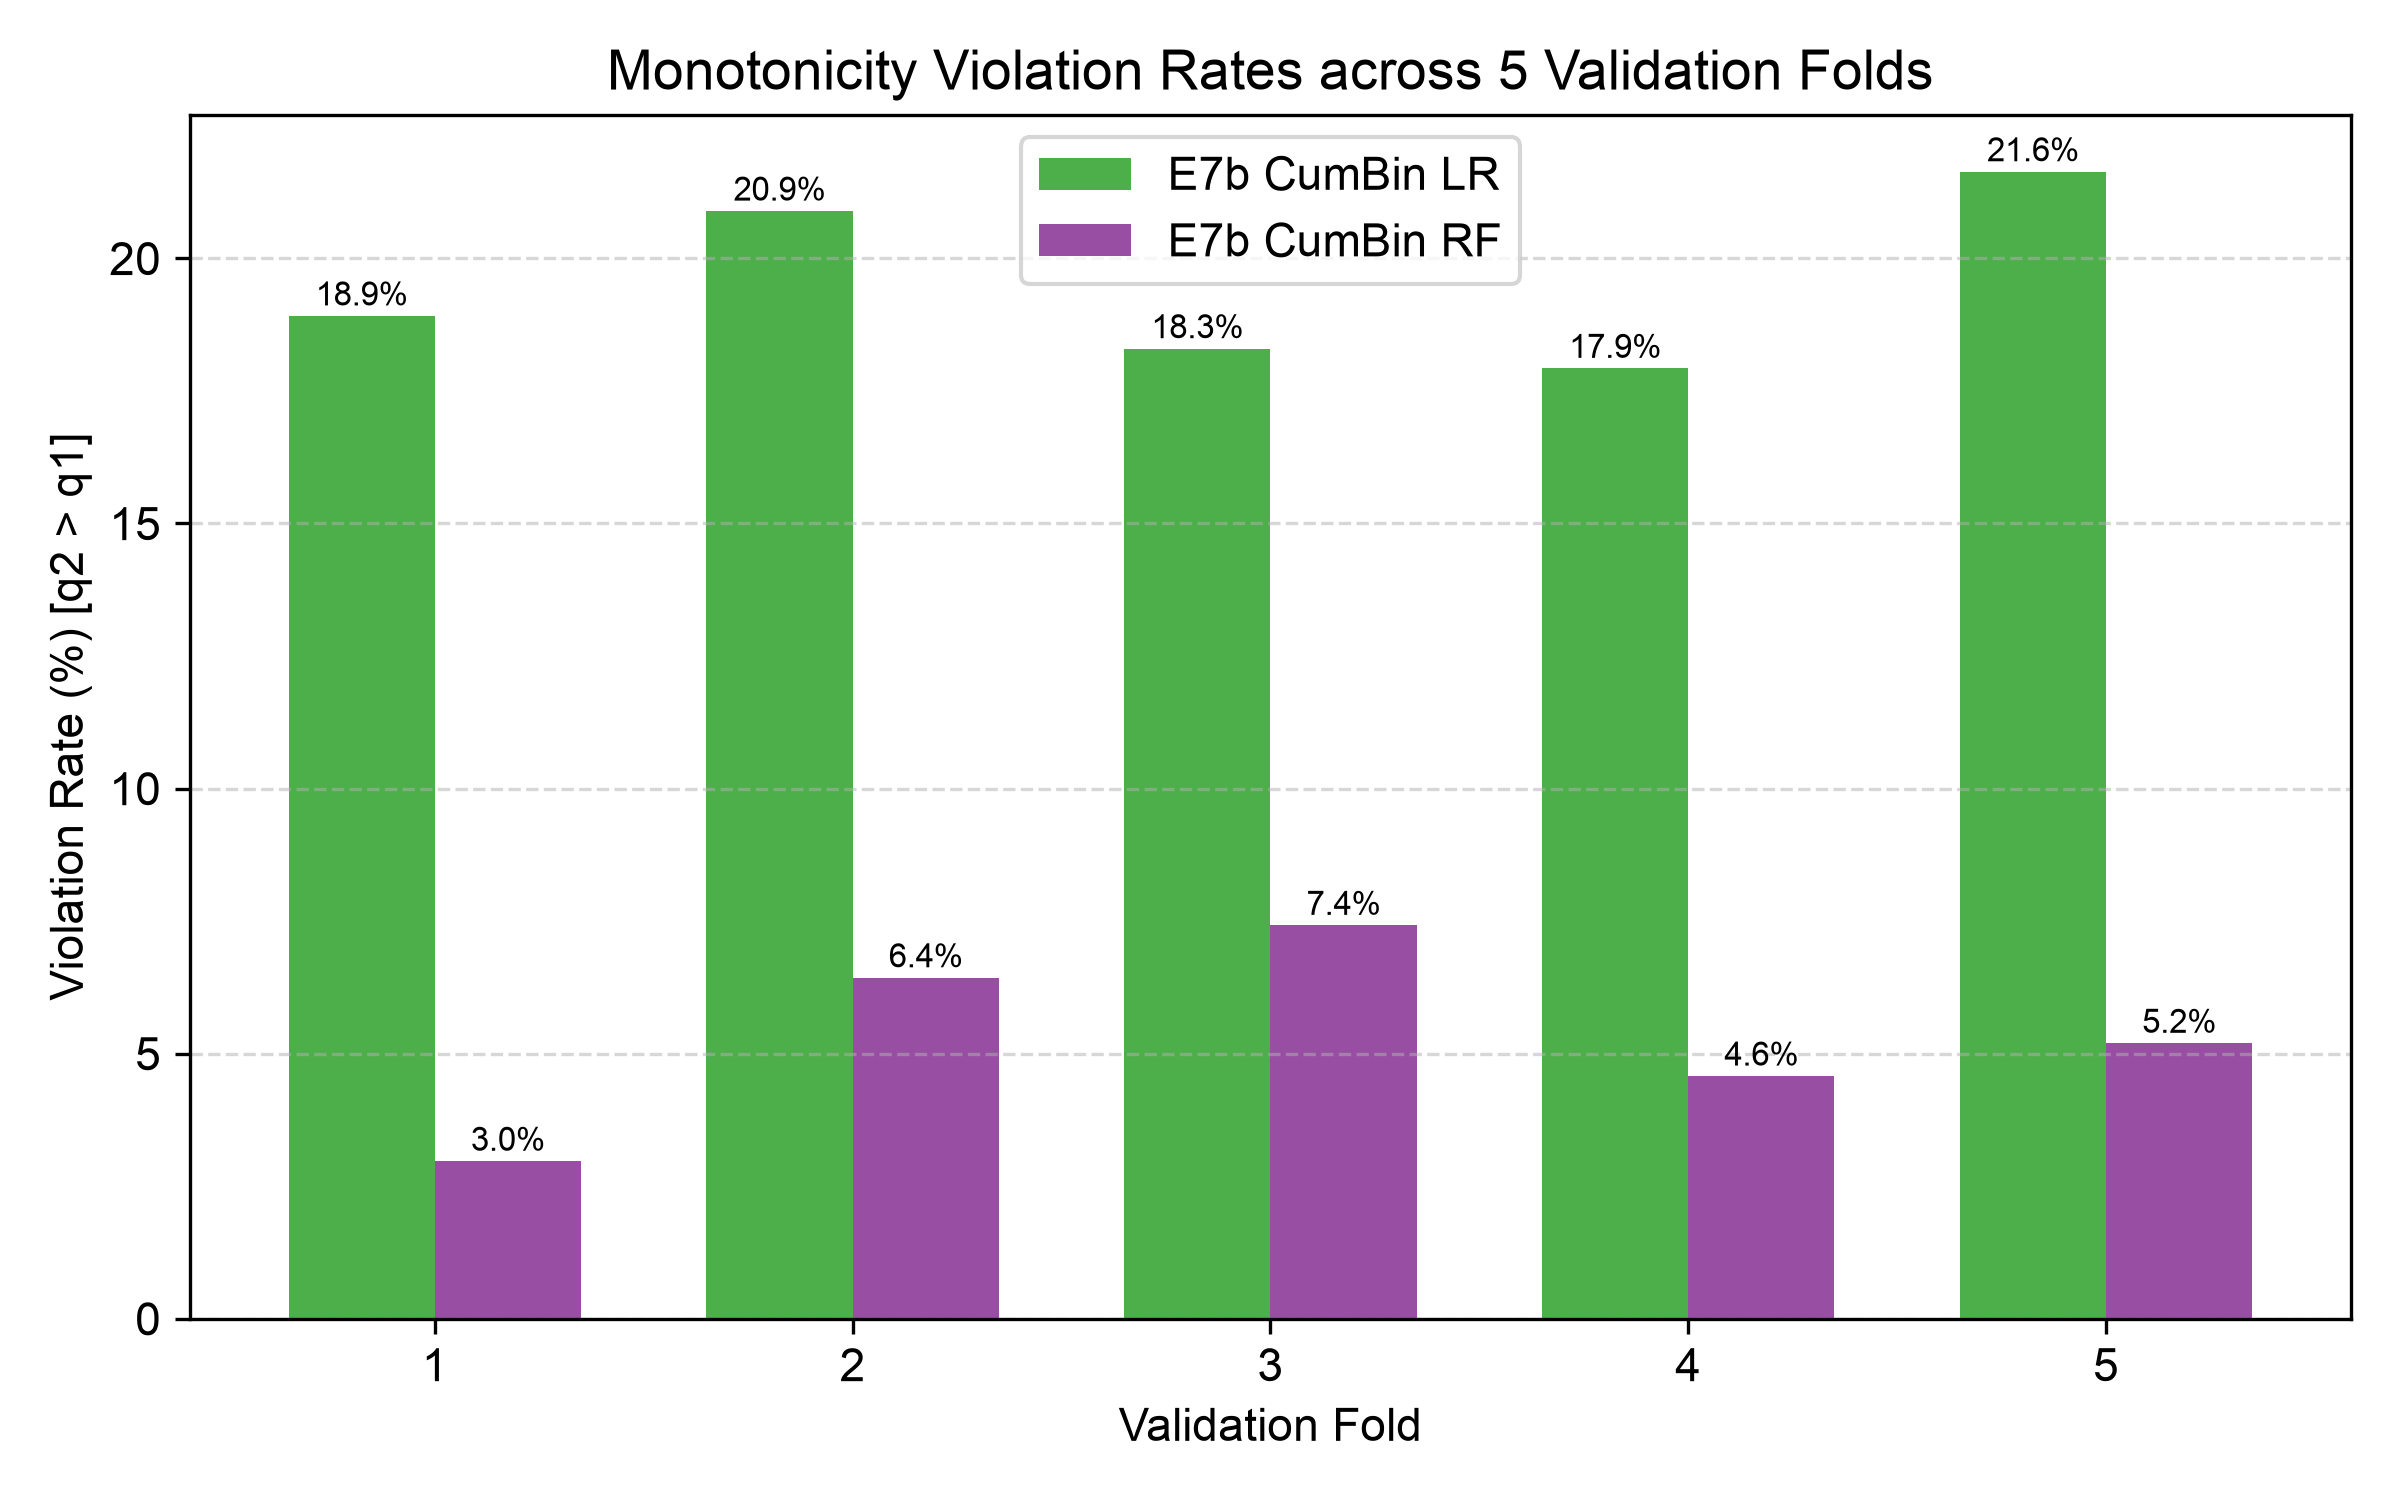
\includegraphics[width=0.75\textwidth]{figures/monotonicity_violation_distribution.png}
\label{fig:monotonicity-violations}
\end{figure}

\textbf{3. Bước đột phá của E7a Balanced:}  
Khi tích hợp \texttt{class\_weight="balanced"}, mô hình \texttt{E7a\_Ordinal\_LogReg\_Balanced} duy trì các siêu phẳng song song tuyệt đối (không bao giờ vi phạm đơn điệu), khôi phục hoàn hảo độ nhạy trên cả ba lớp: Recall $C_0 = 61.24\%$, Recall $C_1 = 32.93\%$, và đạt \textbf{Recall $C_2^+ = 60.37\%$} (cao nhất trong các mô hình cân bằng). Balanced Accuracy thiết lập kỷ lục mới toàn dự án: \textbf{0.5151 $\pm$ 0.0276}.

\section{Bảng so sánh tổng hợp toàn diện (E0 -- E7) trên Legacy Cohort}
\label{sec:so-sanh-tong-hop-e0-e7}

Bảng \ref{tab:master-comparison} tổng hợp toàn bộ 10 mô hình đại diện cho ba trường phái học máy trên cùng tập Legacy Development ($N = 4.045$, Stratified 5-Fold CV cố định). Hình \ref{fig:master-mae-f1} trực quan hóa mối tương quan giữa Macro-F1 và Class MAE, và Hình \ref{fig:master-2step} so sánh chi tiết các lỗi 2 mức nghiêm trọng.

\begin{table}{Bảng so sánh tổng hợp toàn diện các mô hình ($E_0 \to E_7$) trên Legacy Cohort ($N = 4.045$)}
\centering
\small
\label{tab:master-comparison}
\begin{tabularx}{\textwidth}{l p{3.2cm} c c c c c c c}
\toprule
\textbf{Nhóm} & \textbf{Mô hình} & \textbf{Macro-F1} & \textbf{BalAcc} & \textbf{Acc (\%)} & \textbf{MAE} & \textbf{Rec $C_1$} & \textbf{Rec $C_2^+$} & \textbf{$C_2^+ \to C_0$} \\
\midrule
\textbf{Flat} & $E_0$ (Flat RF) & 0.4354 & 0.4667 & 64.10\% & 0.4638 & 16.29\% & 47.32\% & 108 ca \\
\midrule
\multirow{4}{*}{\textbf{Hard}} 
  & $E_1$ (Hard RF--RF) & 0.4550 & 0.4745 & 68.08\% & 0.4133 & 16.46\% & 43.74\% & 120 ca \\
  & $E_2$ (Hard Tuned)  & \textbf{0.4586} & 0.4902 & 65.32\% & 0.4280 & 25.69\% & 39.63\% & 95 ca \\
  & $E_3a$ (Hard RF--LR)& 0.4567 & 0.4964 & 68.43\% & 0.4195 & 11.75\% & 55.00\% & 120 ca \\
  & $E_3b$ (Hard RF--XGB)& 0.4575 & 0.4856 & 68.23\% & 0.4180 & 16.77\% & 44.76\% & 120 ca \\
\midrule
\multirow{2}{*}{\textbf{Soft}} 
  & $E_4$ (Soft RF--RF) & 0.4206 & 0.4309 & 73.75\% & 0.3530 & 5.18\% & 30.19\% & 227 ca \\
  & $E_5$ (Soft RF--LR) & 0.4270 & 0.4506 & 73.37\% & 0.3619 & 3.45\% & 39.13\% & 211 ca \\
\midrule
\textbf{Cost} & $E_6b$ (Soft Cost M1) & 0.4521 & 0.5025 & 56.84\% & 0.5197 & \textbf{34.64\%} & 54.23\% & \textbf{62 ca} \\
\midrule
\multirow{4}{*}{\textbf{Ordinal}} 
  & $E_{7a}$ (OLR Unweighted)& 0.3846 & 0.4002 & \textbf{75.23\%} & \textbf{0.3377} & 0.00\% & 22.00\% & 305 ca \\
  & $E_{7a}$ (OLR Balanced)  & 0.4518 & \textbf{0.5151} & 56.69\% & 0.5382 & 32.93\% & \textbf{60.37\%} & 68 ca \\
  & $E_{7b}$ (CumBin LR)     & 0.3761 & 0.4949 & 63.41\% & 0.5718 & 0.00\% & \textbf{72.88\%} & 106 ca \\
  & $E_{7b}$ (CumBin RF)     & 0.4191 & 0.4900 & 72.34\% & 0.3953 & 0.16\% & 57.30\% & 167 ca \\
\bottomrule
\end{tabularx}
\end{table}

\begin{figure}{Biểu đồ phân tán so sánh Macro-F1 (cao hơn là tốt hơn) và Class MAE (thấp hơn là tốt hơn)}
\centering
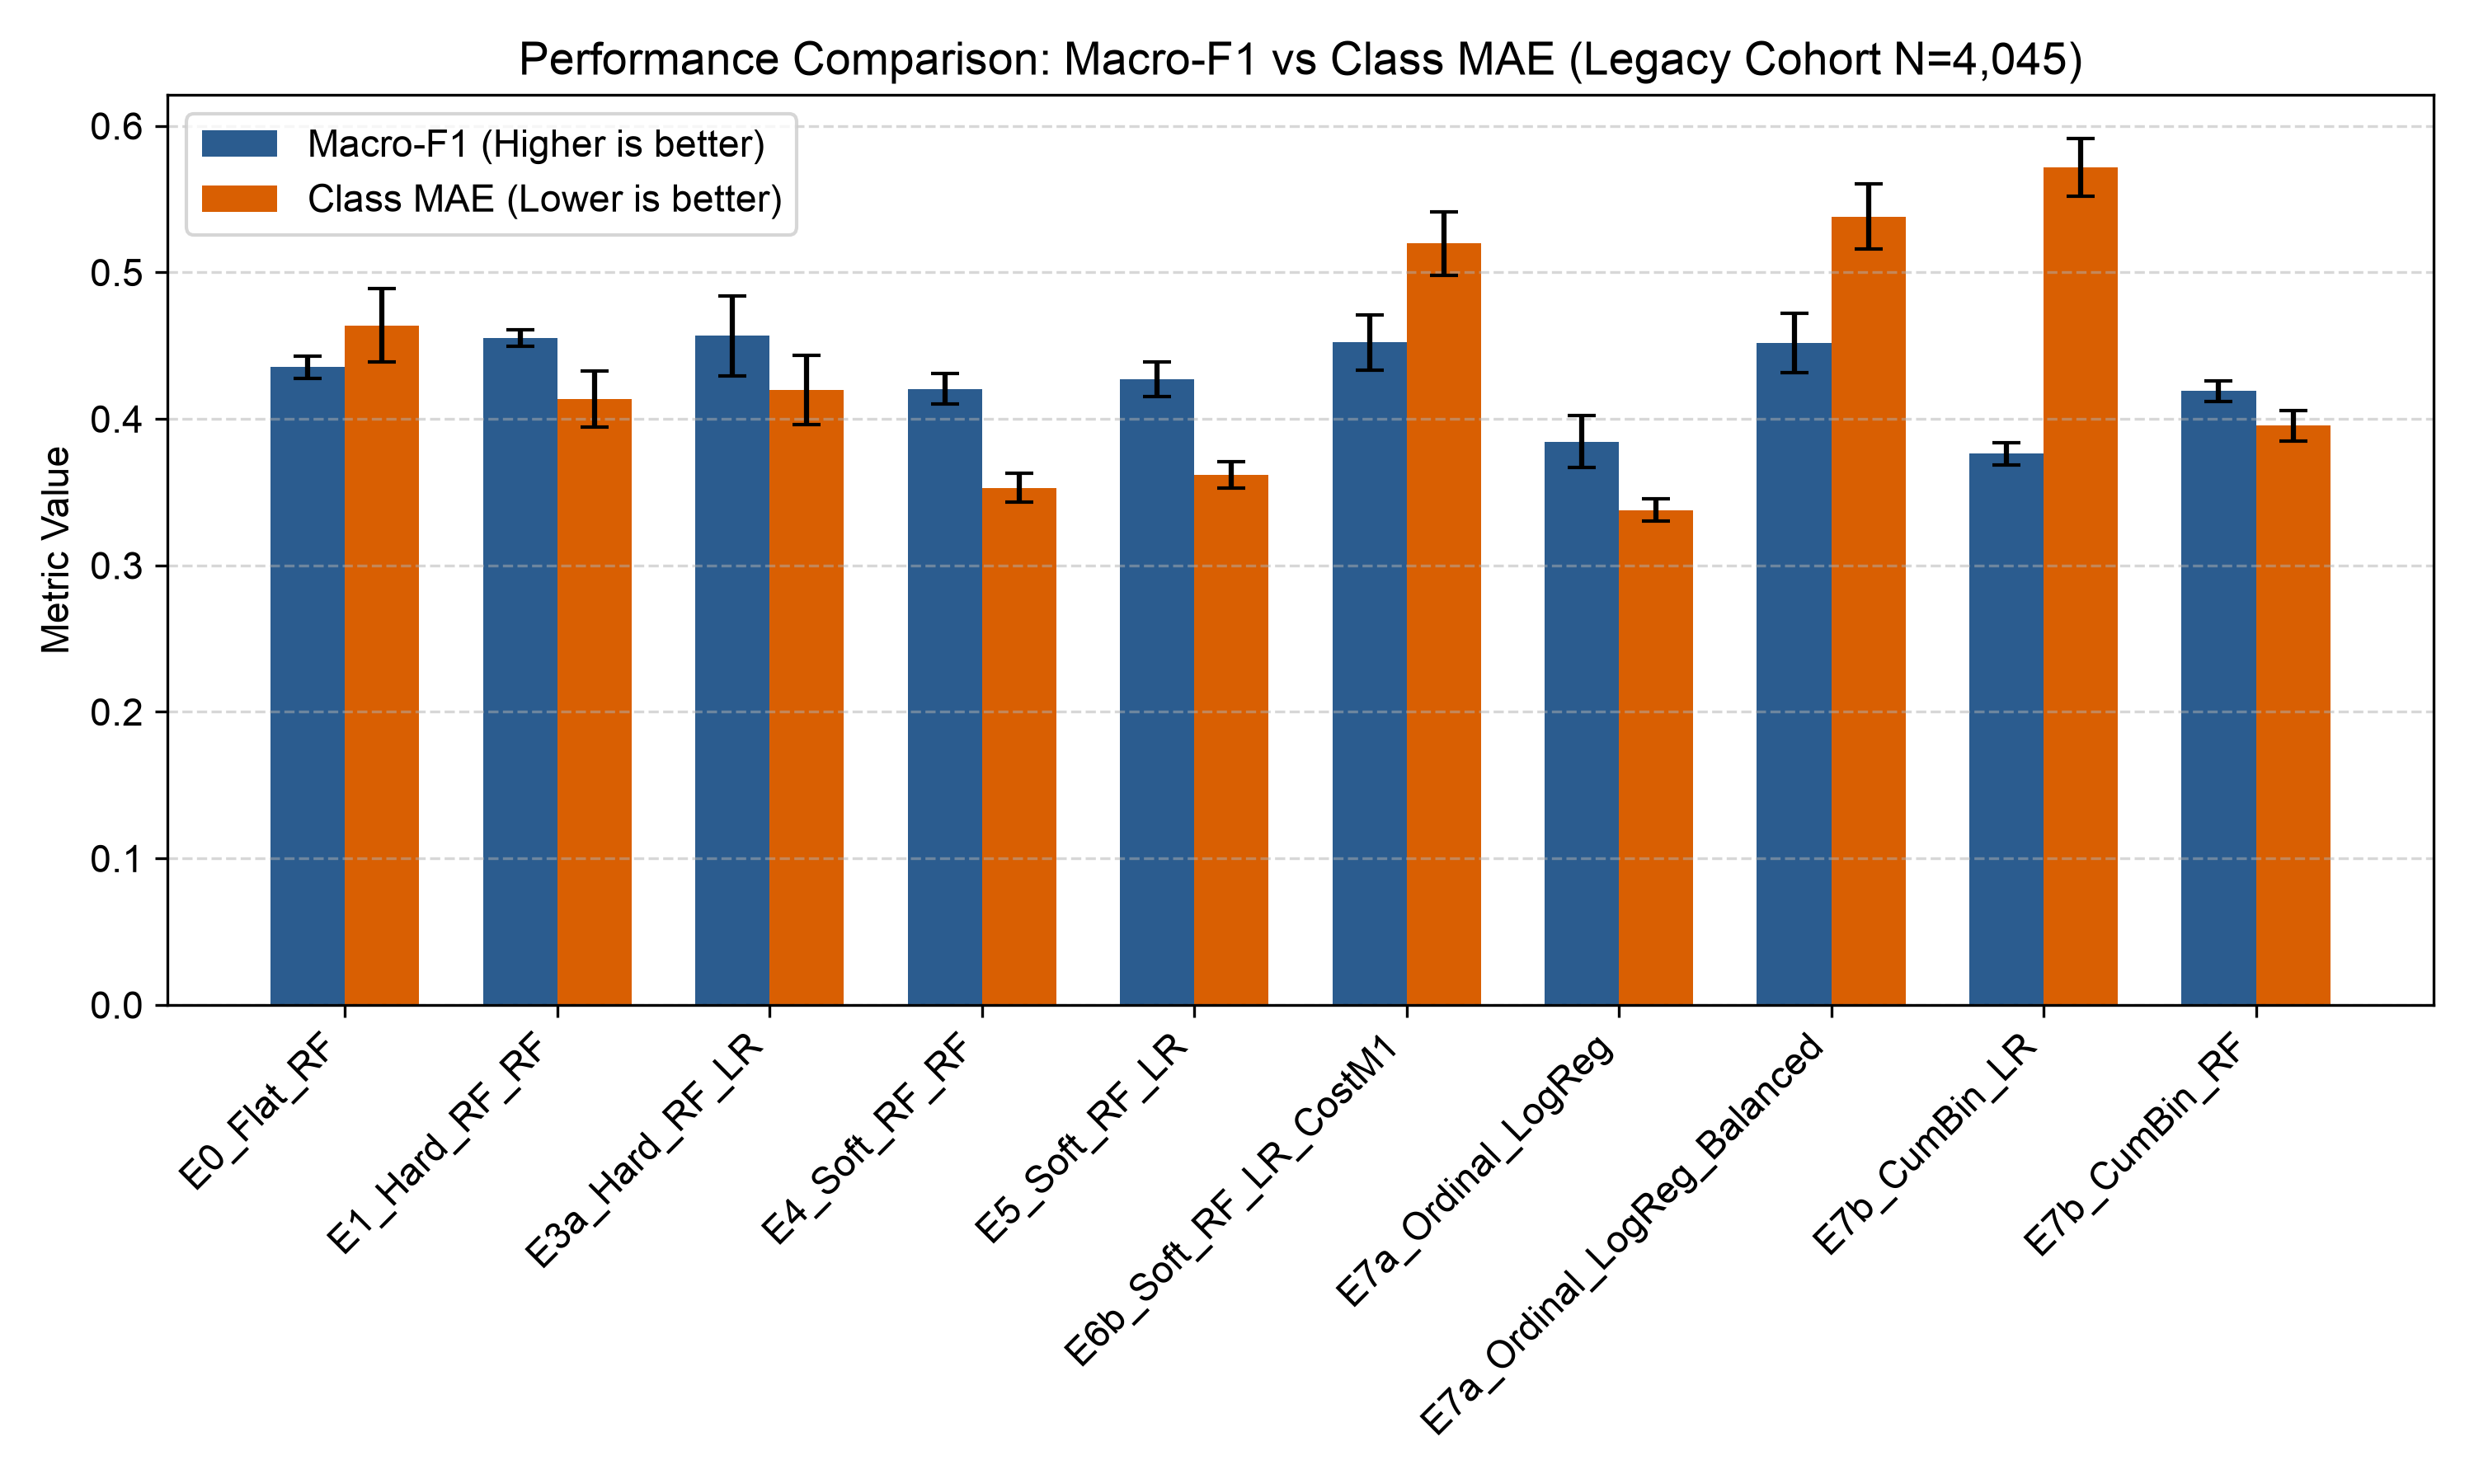
\includegraphics[width=0.88\textwidth]{figures/macro_f1_vs_mae.png}
\label{fig:master-mae-f1}
\end{figure}

\begin{figure}{So sánh số ca sai lệch nghiêm trọng 2 mức: Bỏ sót nặng ($C_2^+ \to C_0$) vs Báo động giả ($C_0 \to C_2^+$)}
\centering
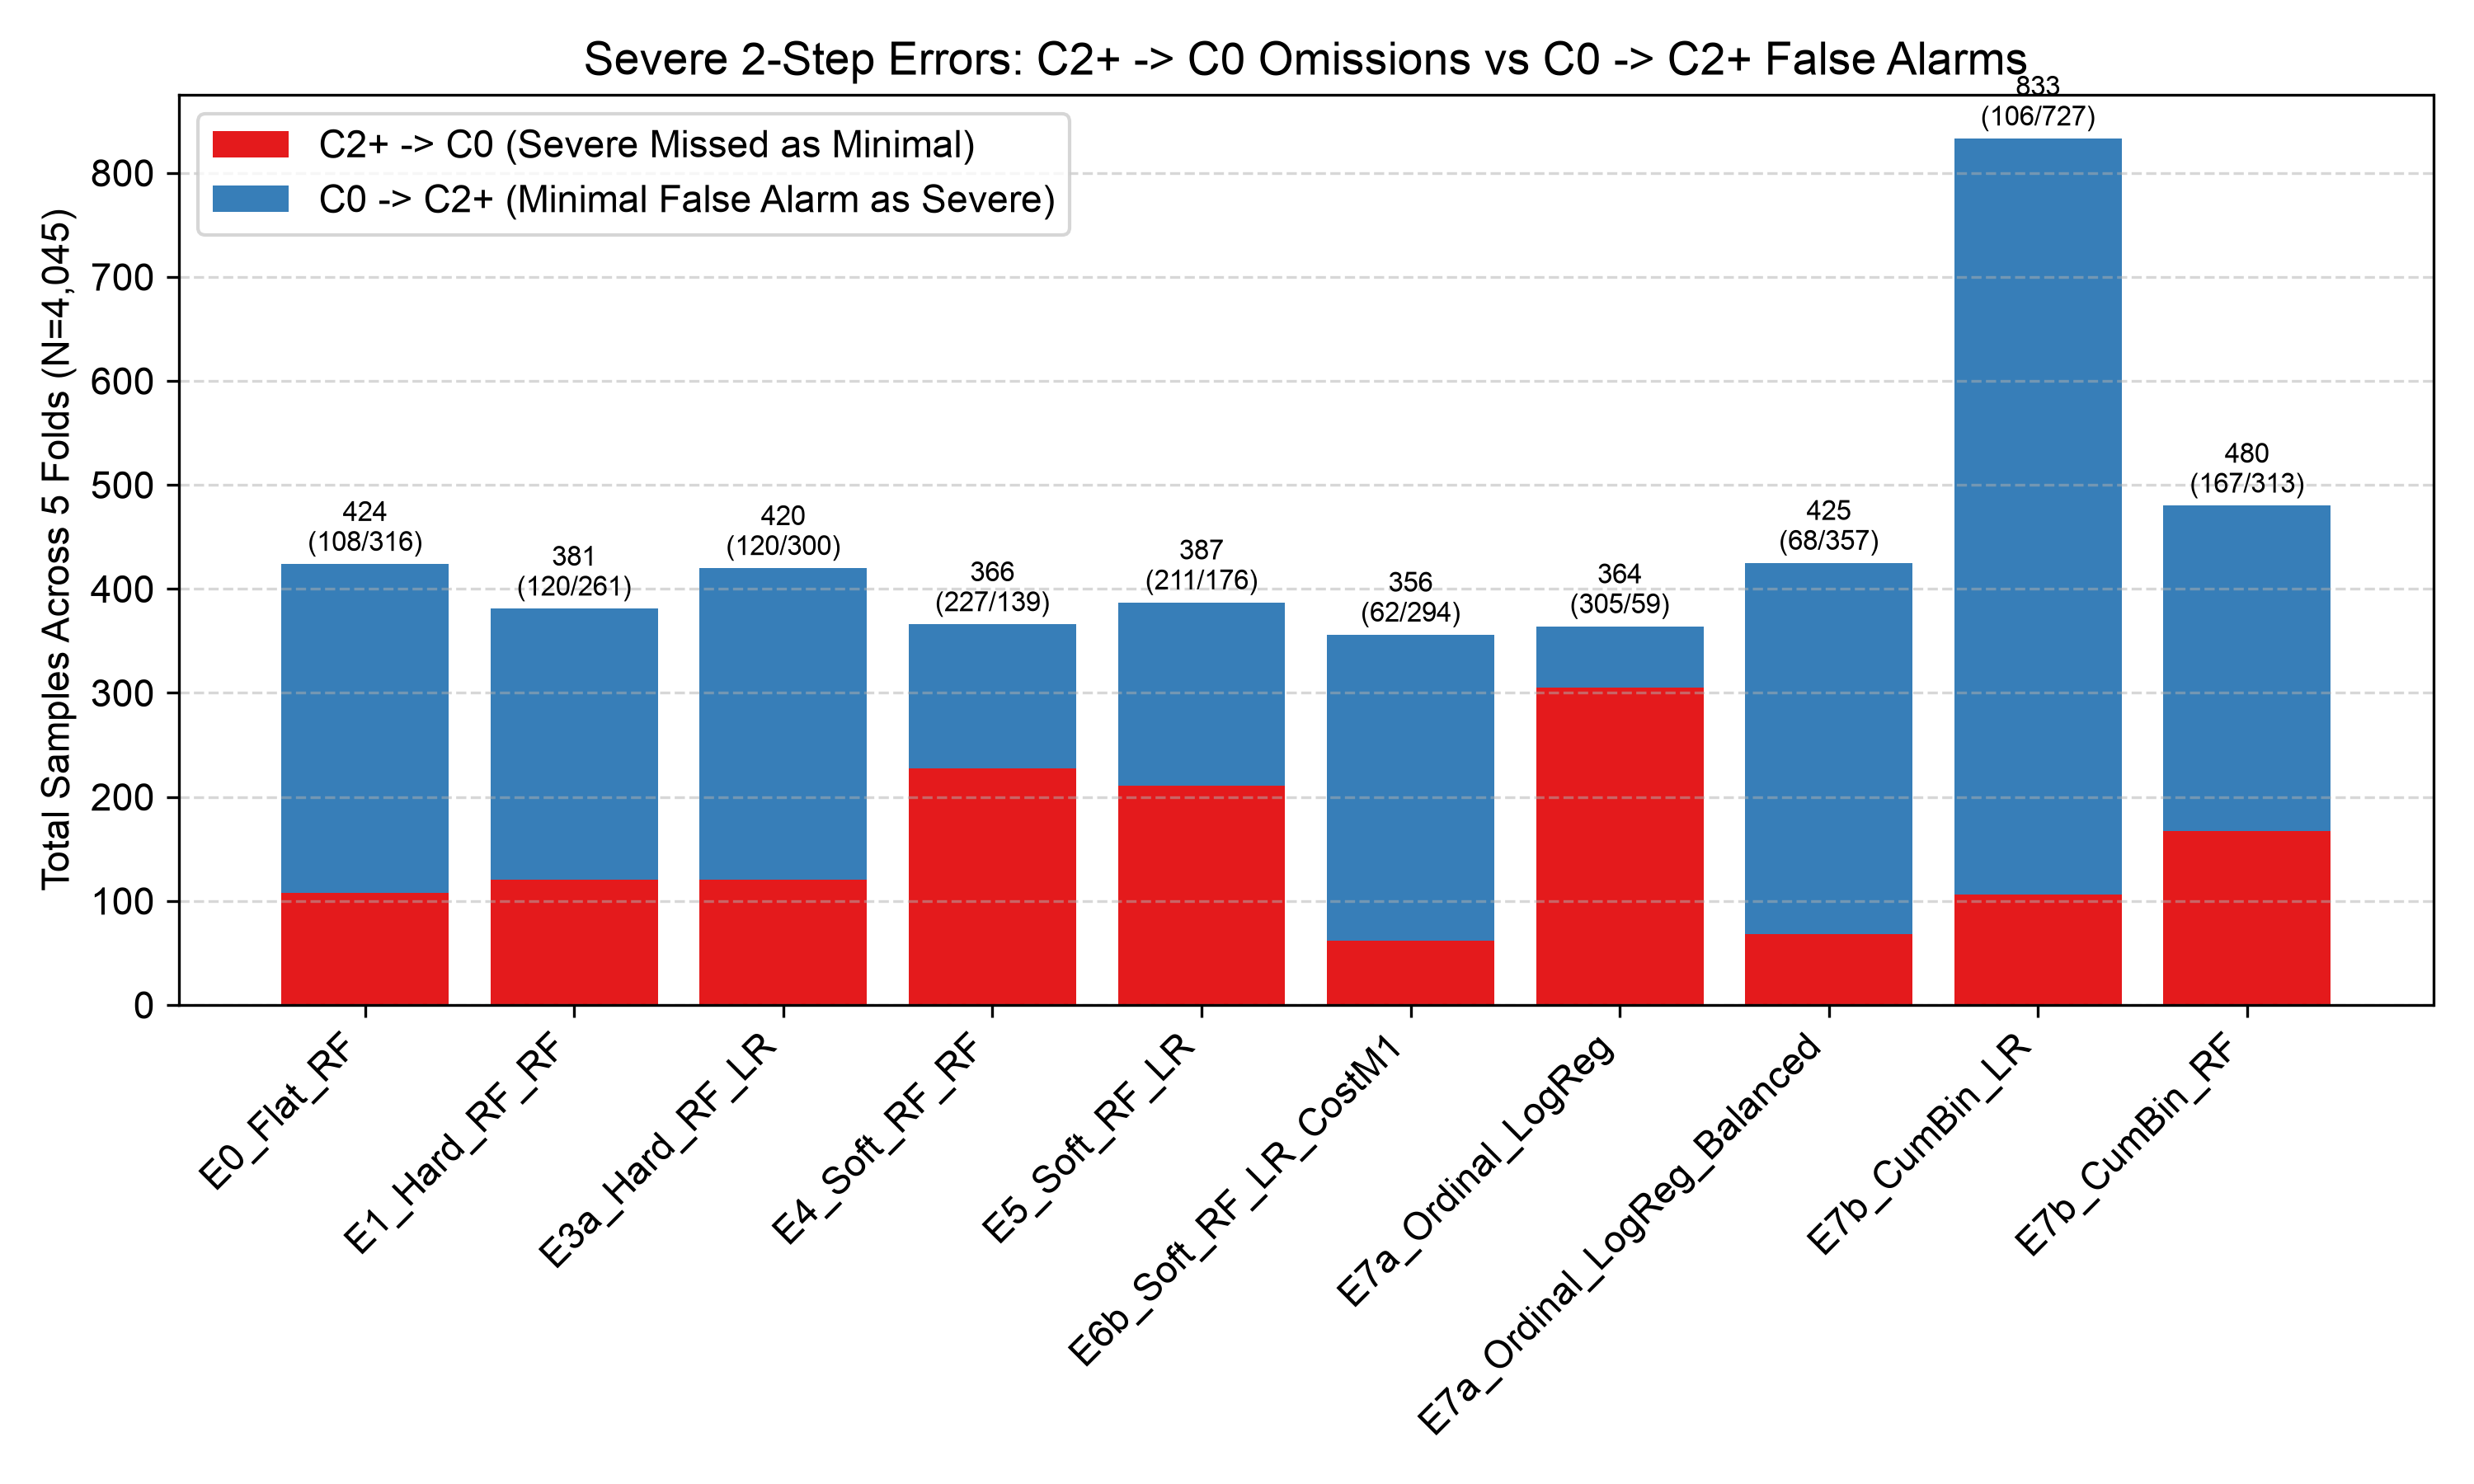
\includegraphics[width=0.88\textwidth]{figures/2step_error_comparison.png}
\label{fig:master-2step}
\end{figure}

\begin{figure}{So sánh ma trận nhầm lẫn Out-of-fold của các mô hình đại diện then chốt trên Legacy Cohort}
\centering
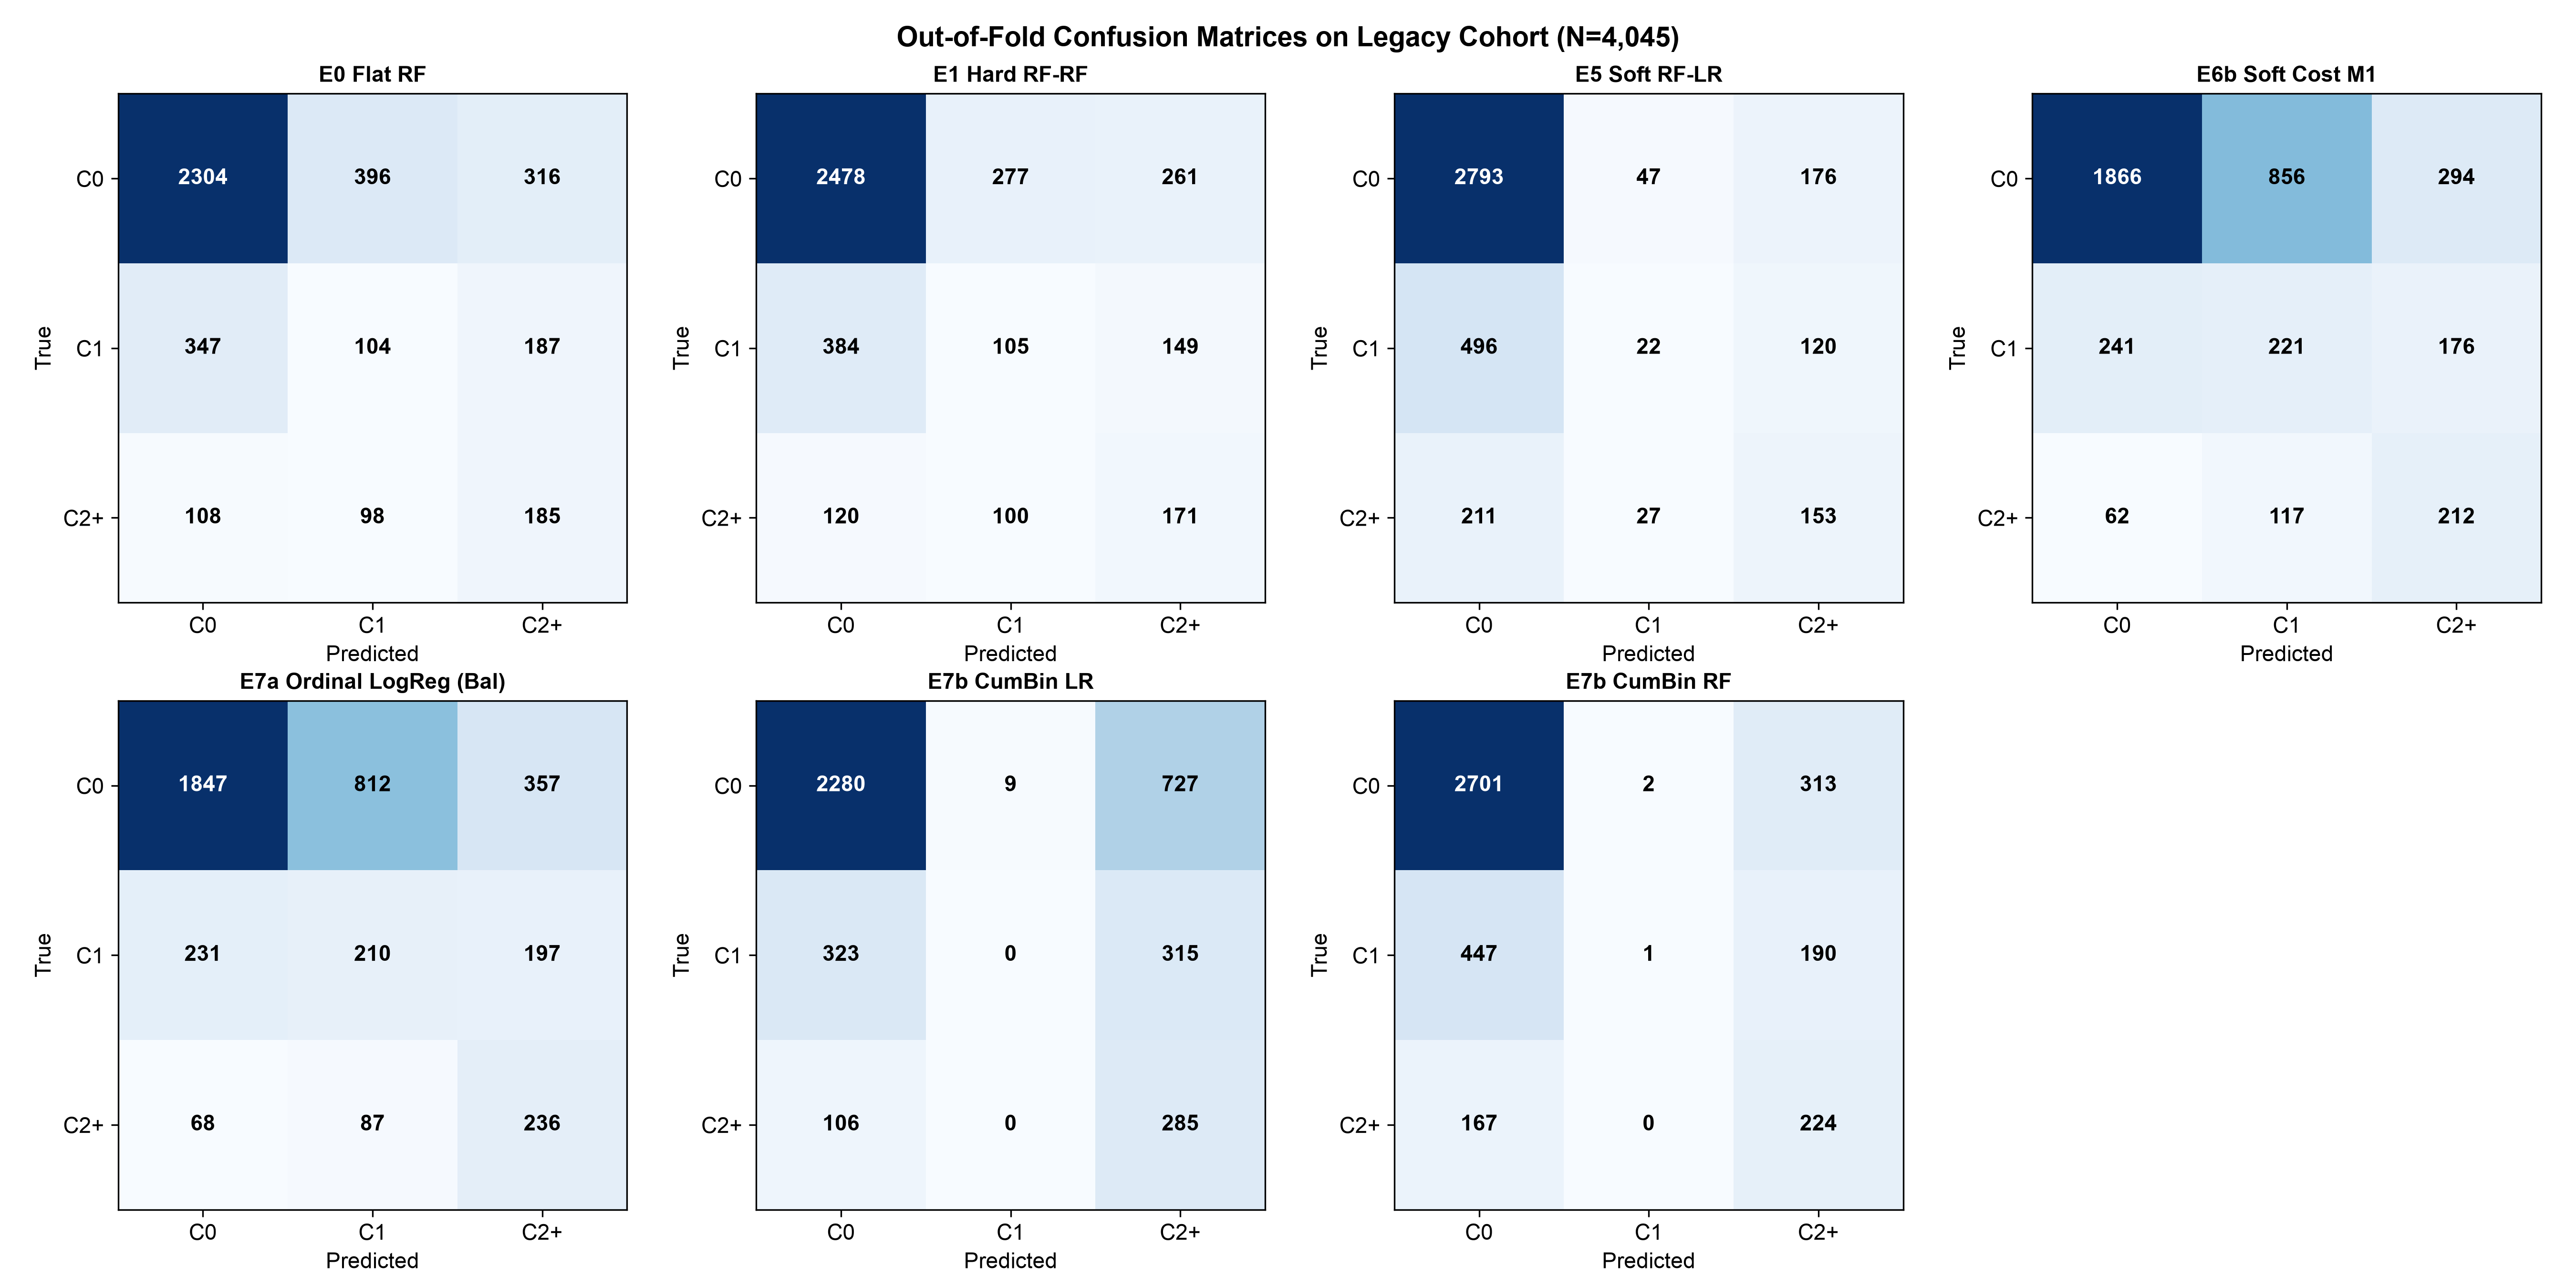
\includegraphics[width=0.95\textwidth]{figures/confusion_matrices_comparison.png}
\label{fig:master-cms}
\end{figure}

\section{Phân tích chuyên sâu về hiệu năng và Đánh giá phản biện}
\label{sec:phan-tich-hieu-nang-thap}

Một câu hỏi cốt lõi mà bất kỳ nhà nghiên cứu hoặc hội đồng phản biện nào cũng sẽ đặt ra khi xem xét kết quả của DepSev-ML:  
\begin{quote}
\textit{“Tại sao các mô hình học máy phức tạp (Ensemble, Hierarchical, Cost-Sensitive, Ordinal) chỉ đạt Macro-F1 trong khoảng $0.43 - 0.46$ và Accuracy chỉ đạt $56\% - 68\%$, trong khi một mô hình ngây thơ (Majority Baseline) dự đoán toàn bộ là $C_0$ có thể đạt Accuracy lên tới $74.56\%$?”}
\end{quote}

Để trả lời câu hỏi này một cách khoa học và thuyết phục, nghiên cứu đưa ra ba luận điểm phân tích thực nghiệm sâu sắc:

\subsection{Sự đánh lừa của chỉ số Accuracy trên dữ liệu mất cân bằng}
Mô hình Majority-Class Baseline gán nhãn dự đoán $\hat{y} = 0$ cho 100\% các quan sát. Trên tập Legacy Development Cohort ($N = 4.045$), mô hình này đạt:
\begin{itemize}
    \item $\text{Accuracy} = 3016 / 4045 = \mathbf{74.56\%}$.
    \item $\text{Macro-F1} = \frac{1}{3} \left( \frac{2 \times 0.7456 \times 1.0}{0.7456 + 1.0} + 0 + 0 \right) = \mathbf{0.2847}$.
    \item $\text{Balanced Accuracy} = \frac{1}{3} (1.0 + 0.0 + 0.0) = \mathbf{0.3333}$.
    \item $\text{Recall } C_1 = \mathbf{0.00\%}$; $\text{Recall } C_2^+ = \mathbf{0.00\%}$.
\end{itemize}

Về mặt ứng dụng y tế, Majority-Class Baseline hoàn toàn \textbf{vô giá trị} vì nó bỏ sót 100\% các ca có triệu chứng trầm cảm ($1.029$ ca bệnh nhân). Nếu một hệ thống y tế chỉ nhìn vào Accuracy để đánh giá, nó sẽ ưu tiên chọn một mô hình không có khả năng phát hiện bệnh!

Ngược lại, mô hình \texttt{E7a\_Ordinal\_LogReg\_Balanced} dù có Accuracy là $56.69\%$ (thấp hơn 74.56\%), nhưng đạt \textbf{Balanced Accuracy = 51.51\%} (cao hơn 33.33\% tới +18.2\%) và nhận diện được \textbf{60.37\% các ca bệnh nặng} ($C_2^+$) cùng \textbf{32.93\% các ca nhẹ} ($C_1$). Đây chính là giá trị thực tiễn đích thực của học máy có kiểm soát.

\subsection{Bản chất sinh học của hiện tượng chồng lấn đặc trưng (Feature Overlap)}
Trầm cảm là một hội chứng tâm thần kinh phức tạp có căn nguyên đa yếu tố (gen di truyền, sang chấn tâm lý xã hội, môi trường sống, sự mất cân bằng chất dẫn truyền thần kinh Serotonin/Dopamine trong não bộ). Các chỉ số sinh lý ngoại vi (như huyết áp, men gan, mỡ máu, chỉ số đường huyết) chỉ phản ánh các biến đổi chuyển hóa gián tiếp đi kèm. 

Hiện tượng diện tích chồng lấn Bayes $\Omega_{\text{overlap}}$ giữa người bình thường ($C_0$) và người trầm cảm nhẹ ($C_1$) rất lớn (Hình \ref{fig:overlap-pca}) tạo nên một \textbf{trần hiệu năng tự nhiên (Performance Ceiling)} trong khoảng Macro-F1 từ $0.45$ đến $0.46$. Không có bất kỳ thuật toán nào có thể vượt qua trần hiệu năng này nếu chỉ thuần túy sử dụng các biến số sinh lý hiện có mà không bổ sung các dữ liệu chuyên sâu hơn (như gen, nồng độ Cortisol huyết thanh, hoặc dữ liệu hành vi di động liên tục).

\subsection{Bản đồ đánh đổi và tính không thể thay thế tuyệt đối}
Thực nghiệm khẳng định không có một mô hình nào là tối ưu toàn diện trên mọi thước đo:
\begin{itemize}
    \item Nếu ưu tiên \textbf{Accuracy cao nhất và MAE thấp nhất}: Chọn \texttt{E7a Unweighted} (Acc 75.23\%, MAE 0.3377), nhưng phải chấp nhận mất hoàn toàn nhóm nhẹ $C_1$.
    \item Nếu ưu tiên \textbf{Macro-F1 cao nhất}: Chọn \texttt{E2} (Macro-F1 0.4586) hoặc \texttt{E3a} (0.4567), nhưng phải chấp nhận 120 ca nặng bị tắc nghẽn ở Giai đoạn 1.
    \item Nếu ưu tiên \textbf{An toàn lâm sàng, giảm thiểu tối đa ca bỏ sót nặng}: Chọn \texttt{E6b} (chỉ bỏ sót 62 ca $C_2^+ \to C_0$).
    \item Nếu ưu tiên \textbf{Cân bằng đa lớp toàn diện và nhận diện ca nặng tốt nhất}: Chọn \texttt{E7a\_Ordinal\_LogReg\_Balanced} (Balanced Accuracy 0.5151, Recall $C_2^+ = 60.37\%$).
\end{itemize}

\section{Thảo luận và Trả lời các câu hỏi nghiên cứu}
\label{sec:thao-luan-rq}

\begin{itemize}
    \item \textbf{Trả lời RQ1:} Nhóm xét nghiệm cận lâm sàng máu ($F_2$) và lối sống ($F_3$) đóng góp thực chất nhất vào mức tăng hiệu năng (+14\% đến +23\% Macro-F1 so với chỉ dùng dấu hiệu sinh tồn $F_1$). Việc kết hợp toàn diện $F_4$ mang lại lợi thế lớn nhất khi mô hình được tinh chỉnh siêu tham số có kiểm soát.
    \item \textbf{Trả lời RQ2:} Hiệu năng suy giảm mạnh nhất tại bước chuyển $T_2 \to T_3$ (Macro-F1 giảm 34.4\%), với điểm nghẽn tập trung tại ranh giới phân tách lớp nhẹ $C_1$ do sự chồng lấn phân phối sinh lý với lớp bình thường $C_0$.
    \item \textbf{Trả lời RQ3:} Mở rộng dữ liệu lên 3 chu kỳ NHANES ($N = 14.581$) giúp ổn định phân phối của các lớp hiếm $C_3/C_4$, nhưng không giúp cải thiện Macro-F1 tổng thể do trần chồng lấn đặc trưng.
    \item \textbf{Trả lời RQ4:} Phân loại phân cấp hai tầng cứng cải thiện nhẹ Macro-F1 (+0.02 so với Flat RF) nhưng gây ra hiện tượng lan truyền sai số nghiêm trọng khi loại bỏ nhầm 30.7\% số ca bệnh nặng ở Giai đoạn 1.
    \item \textbf{Trả lời RQ5:} Mô hình Soft Hierarchical nhạy chi phí ($E_6b$) và Ordinal Logistic Regression cân bằng ($E_7a$) đã giải quyết triệt để sự tắc nghẽn của cổng cứng, giảm thiểu số ca bỏ sót nặng xuống còn 62--68 ca, thiết lập kỷ lục Balanced Accuracy 0.5151 và duy trì độ bền vững trên tập kiểm tra theo dòng thời gian (Branch D, Balanced Accuracy = 0.5073).
\end{itemize}
\cleardoublepage
